% This is LLNCS.DEM the demonstration file of
% the LaTeX macro package from Springer-Verlag
% for Lecture Notes in Computer Science,
% version 2.3 for LaTeX2e
%
\documentclass{llncs}
%
\usepackage{makeidx}  % allows for indexgeneration
\usepackage[pdftex]{graphicx}
\usepackage{multicol}
\usepackage{url}
\usepackage{subfigure}
%\usepackage{latex8}
%

% Make floats work with multicols (maybe)
\makeatletter
\newenvironment{figurehere}
	{\def\@captype{figure}}
	{}
\makeatother

\begin{document}
%
%\frontmatter          % for the preliminaries
%
\pagestyle{headings}  % switches on printing of running heads
\addtocmark{Model-Based Integration} % additional mark in the TOC
%
%\tableofcontents
%
\mainmatter              % start of the contributions
%
\title{Towards Model-Based Integration of Tools and Techniques for Embedded Control System
Design, Verification, and Implementation}
%
\titlerunning{Model-Based Integration}  % abbreviated title (for running head)
%                                     also used for the TOC unless
%                                     \toctitle is used
%
\author{Joseph Porter \and G\'{a}bor Karsai \and P\'{e}ter V\"{o}lgyesi \and Harmon Nine \and Peter Humke \and Graham Hemingway \and Ryan Thibodeaux \and J\'{a}nos Sztipanovits}
%
\authorrunning{Joseph Porter et al.}   % abbreviated author list (for running head)
%
%%%% list of authors for the TOC (use if author list has to be modified)
\tocauthor{Joseph Porter}
%
\institute{Institute for Software Integrated Systems, \\Vanderbilt University, \\Nashville TN 37203, USA,\\
\email{jporter@isis.vanderbilt.edu},\\ WWW home page:
\texttt{http://www.isis.vanderbilt.edu}
}

\maketitle              % typeset the title of the contribution

\begin{abstract}
While design automation for hardware systems is quite advanced, this is not the case for practical embedded systems. The current state-of-the-art is to use a software modeling environment and integrated development environment for code development and debugging, but these rarely include the sort of automatic synthesis and verification capabilities available in the VLSI domain. We present a model-based integration environment which uses a graphical architecture description language (EsMoL) to pull together control design, code and configuration generation, platform-specific resimulation, and a number of other features useful for taming the heterogeneity inherent in safety-critical embedded control system designs.  We describe concepts, elements, and development status for this suite of tools.
\end{abstract}
%
%\twocolumn
%\begin{multicols}{2}

\section{Introduction}
\section{Introduction}

High confidence embedded control system software designs often require formal 
analyses to ensure design correctness.  Detailed models of system behavior 
include numerous design concerns, such as controller stability, timing 
requirements, fault tolerance, and deadlock freedom.  Models for each of these
domains must together provide a consistent and faithful representation of the
potential problems an operational system would face.  This poses challenges 
for structural representation of models, as components and design
aspects are commonly tightly coupled.  The ESMoL language is built on a platform which provides inherent correctness properties for well-formed models.  The properties include functional determinism, deadlock freedom, and timing determinism.  We also rely on decoupling
methods such as passive control design (decoupling controller stability from
network effects) and time-triggered models of computation (decoupling timing 
and fault tolerance from functional requirements) and on compositional 
and incremental analysis to enable rapid prototyping in our design environment.  As design paradigms become more fully decoupled and analysis becomes faster (and therefore cheaper), we move closer to the goal of ``correct by construction'' model-based software 
development.

In compositional analysis for graphical software models, sometimes the nature of the analysis does not easily lead to a clean syntactic decomposition in the models.  Examples include end-to-end properties such as latency, and other properties which require the evaluation of particular connections spanning multiple levels of components.  One approach for dealing with such properties in hierarchical dataflow designs is the creation of interface data for each component which abstracts properties of that component.  Hierarchical schedulability models defined over dataflows are a particular example\cite{sched:shin} -- each composite task contains a resource interface characterizing the aggregate supply required to schedule the task and all of its children.  Extensions to the formalism allow the designer to efficiently and incrementally evaluate whether new tasks can be admitted to the design without recomputing the full analysis\cite{sched:easwaran}.  One goal is to see whether this approach can be generalized to other properties that do not easily fit the compositional structure of hierarchical designs.
 
One particular syntactic analysis problem concerns synchronous execution environments 
and system assembly.  In dataflow models of computation we are often concerned with 
so-called ``algebraic'' or delay-free processing loops in a design model.  Many
synchronous formalisms require the absence of delay-free loops in order to 
guarantee deadlock freedom \cite{moc:ltta} or timing determinism \cite{moc:sdf}.
This condition can be encoded structurally into dataflow modeling languages --
for example Simulink \cite{tools:mathworks} analyzes for algebraic loops and attempts to resolve them analytically.  In the Ptolemy dataflow design environment, such causality loops 
complicate scheduling requiring fixed-point iteration to ensure convergence of 
results\cite{tools:ptolemy2}. In our work we only consider the structural 
problem of loop detection in model-based distributed embedded system designs.

We propose a simple incremental cycle enumeration technique with the following
characteristics:

\begin{itemize}
\item The algorithm uses Johnson's simple cycle enumeration algorithm as its 
core engine\cite{cycles:johnson75}.  Johnson's algorithm is known to be 
efficient \cite{cycles:mateti76}.  We use cycle enumeration rather than simple
detection in order to provide useful feedback to the designers.
\item The algorithm exploits the component structure of hierarchical dataflow 
models to allow the cycle enumeration to scale up to larger models.   A small amount of interface data is created and stored for each component as the analysis processes the model hierarchy from the bottom up.  The interface data consists of a set of typed graph edges indicating whether dataflow paths exist between each of the component's input/output pairs.  Each component is evaluated for cycles using the interface data instead of the detailed dataflow connections of its child components.
\item   The interface data facilitates incremental analysis, as it also contains a flag to determine whether modifications have been made to the component.  We refer to the flag and the edges as an \emph{incremental interface} for the component.  This is consistent with the use of the concept in other model analysis domains, such as compositional scheduling analysis\cite{sched:easwaran}. In order for the incremental method to assist our development processes, the total runtime for all partial assessments of the model should be no greater than the analysis running on the full model.  Because the amount of interface data supporting the incremental analysis is small, the method should scale to large designs without imposing onerous data storage requirements on the model.
\item The technique will not produce false positive cycle reports, though it 
may compress multiple cycles into a single cycle through the interface abstraction.  Fortunately,
full cycles can be recovered from the abstract cycles through application
of the enumeration algorithm on a much smaller graph.
\end{itemize}

Zhou and Lee presented an algebraic formalism for detecting causality cycles
in dataflow graphs, identifying particular ports that participate in a cycle.
\cite{comp:causality}. Our work traverses the entire model and extracts all 
elementary cycles,
reporting all ports and subsystems involved in the cycle.
Our approach is also inspired by work from Tripakis et al, which 
creates a richer incremental interface for components to capture execution 
granularity as well as potential deadlock information\cite{moc:hsdf}.  
Their approach is lossless, in that it retains sufficient detail to faithfully represent dataflow structure and execution granularity.  It is much more complex in both model space and computation than our approach. Our formalism does not aim to pull 
semantic information forward into the interface beyond connectivity.  In that sense our approach is more general, as it could be applied to multiple 
model analysis problems in the embedded systems design domain.

The KPASSA model analysis tool described by Boucaron et al 
\cite{cycles:boucaron} performs task graph scheduling analysis for 
latency-insensitive synchronous designs.   Their formal model leans heavily on loop structures, and as such one component of their tool relies on an 
implementation of Johnson's cycle enumeration algorithm\cite{cycles:boucaron2}.  Their formal model is specific to a particular model of computation, and their application of cycle checking is only one small component of that solution.




\section{Toolchain Vision and Overview}

\begin{figure}
	\centering
   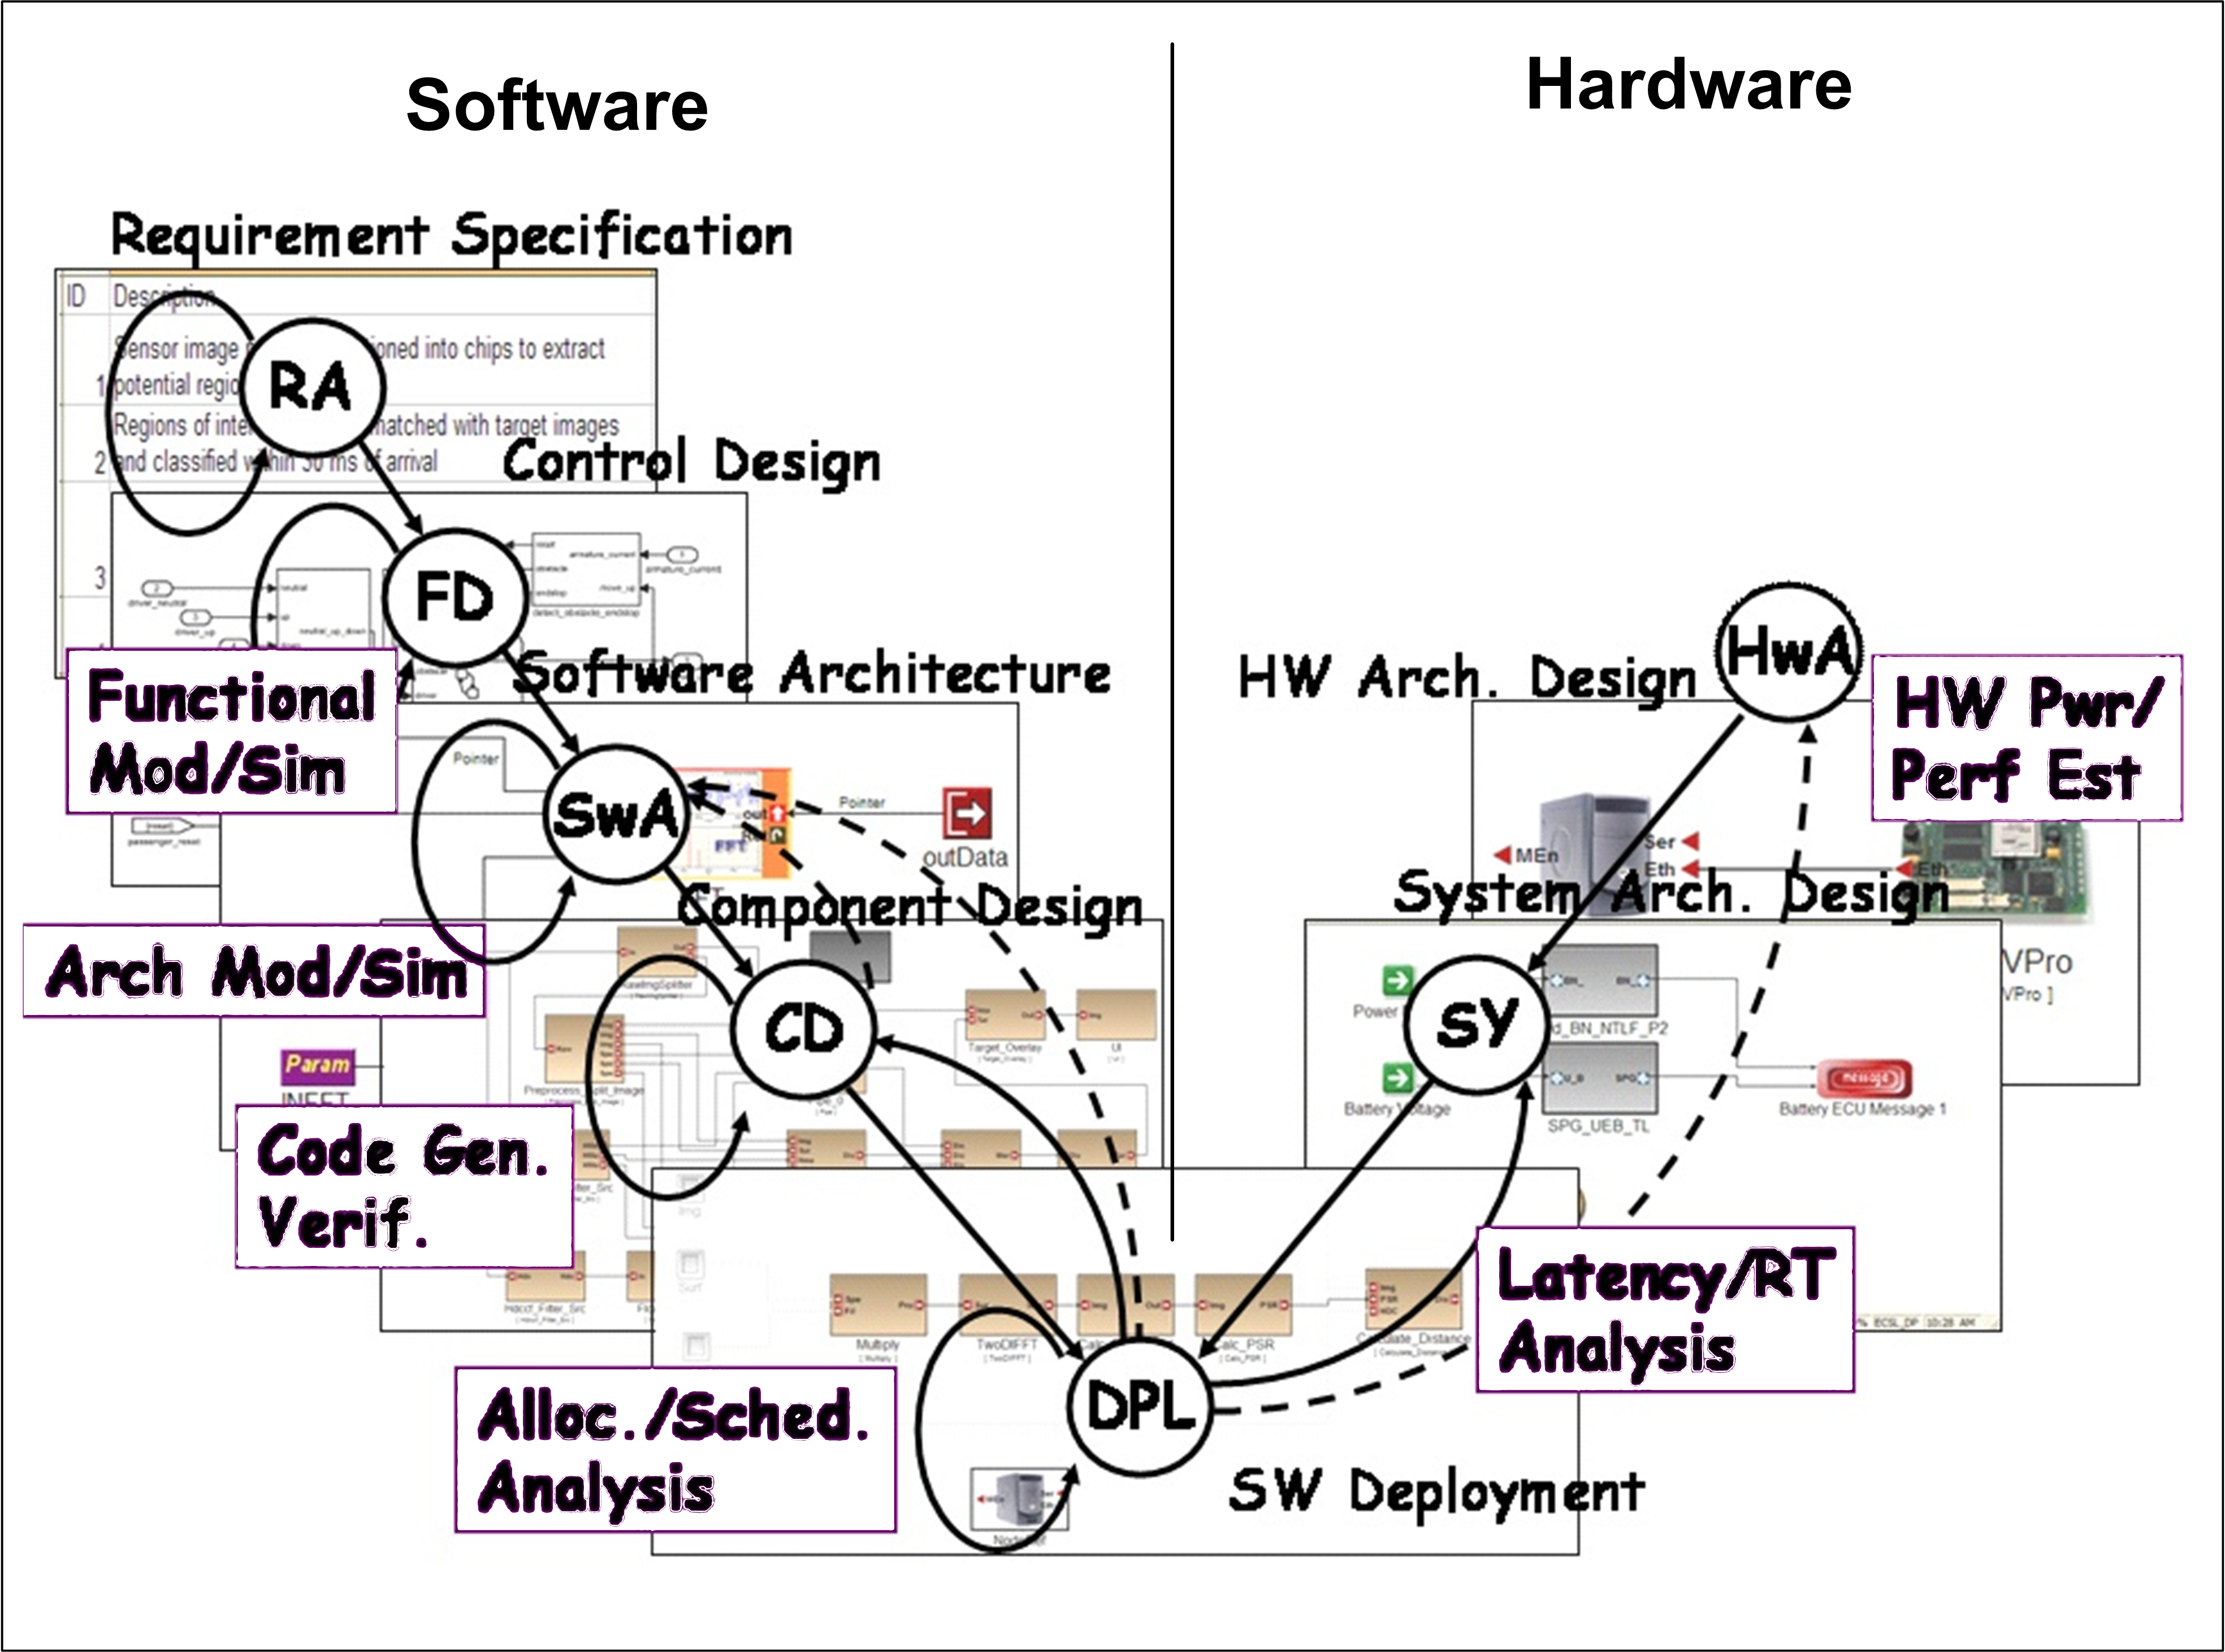
\includegraphics[width=0.65\columnwidth]{diagrams/vdiagram.png}
   \caption{Conceptual model of the toolchain: Development flow}
   \label{fig:vdiagram}
\end{figure}

In this work, we envision a sophisticated, end-to-end toolchain that supports not only construction but also the verification of the engineering artifacts (including software) for high-confidence applications. The development flow provided by the toolchain shall follow a variation of the classical V-model (with software and hardware development on the two branches), with some refinements added at the various stages. Fig. \ref{fig:vdiagram} illustrates this development flow.

Consider the general class of control system designs for use in a flight control system.  Sensors, actuators, and data networks are designed redundantly to mitigate faults.  The underlying hardware implements a variant of the time-triggered architecture (TTA)~\cite{kopetz:2001-22a}, which provides precise timing and reliability guarantees.  Safety-critical tasks and messages execute according to strict precomputed schedules to ensure synchronization between replicated components and provide fault mitigation and management.  Software implementations of the control functions must pass strict certification requirements which impose constraints on the software as well as on the development process.  

A modeling language to support this development flow must have several desired properties:  (1) the ability to capture the relevant aspects of the system architecture and hardware, (2) ability to ``understand'' (and import) functional models from existing design tools, (3) support for componentization of functional models, and (4) ability to model the deployment of the software architecture onto the hardware architecture. The ability to import existing models from functional modeling tools is not a deeply justified requirement, it is merely pragmatic.  EsMoL provides modeling concepts and capabilities that are highly compatible with AADL~\cite{AADL}.  The chief differences are that EsMoL aims for a simpler graphical entry language, a wider range of execution semantics, and most important model-enabled integration to external tools as described below.  Model exchange with AADL tools may be desirable in the future.  A simple sample design will introduce key points of our model-based development flow and illustrate language concepts.  

Our language design was influenced by two factors: (1) the MoC implemented by the platform and (2) the need for integration with legacy modeling and embedded systems tools. We have chosen Simulink/Stateflow as the supported ``legacy'' tool. As our chosen MoC relies on periodically scheduled time-triggered components, it was natural to use this concept as the basis for our modeling language and interpret the imported Simulink blocks as the implementation of these components. To clarify the use of this functionality, we import a Simulink design and select functional subsets which execute in discrete time, and then assign them to software components using a modeling language that has compatible (time-triggered) semantics. Communication links (signals) between Simulink blocks are mapped onto TTA messages passed between the tasks. The resulting language provides a componentized view of Simulink models that are scheduled periodically (with a fixed rate) and communicate using time-triggered messages.  Extensions to heterogeneous MoC-s is an active area of research.

\subsection{Requirements Analysis (RA)}

Our example will model a data network implementing a single sensor/actuator loop with a distributed implementation.  The sensors and actuators in the example are doubly-redundant, while the data network is triply-redundant.  Unlike true safety-critical designs, we will deploy the same functions on all replicas rather than requiring multiple versions as is often done in practice~\cite{DO178B}.  The sensors and actuators close a single physical feedback loop.  Specifying the physical system and particulars of the control functions are beyond the scope of this example as our focus is on modeling.

This example has an informal set of requirements, though our modeling language currently supports the formalization of timing constraints between sensor and actuator tasks.  Formal requirements modeling offers great promise, but in ESMoL requirements modeling is still in conceptual stages.  A simple sensor/actuator latency modeling example appears in a later section covering preliminary features for the language.

\subsection{Functional Design (FD)}

\begin{figure}
	\centering
   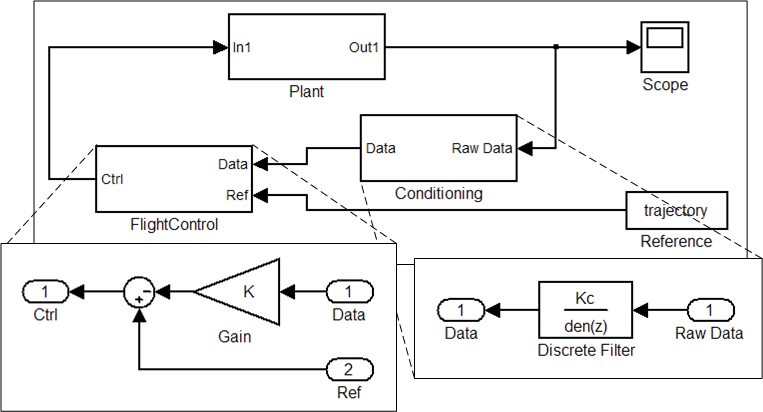
\includegraphics[width=0.65\columnwidth]{diagrams/sl_design.png}
   \caption{Simulink design of a basic signal conditioner and controller.}
   \label{fig:sl_design}
\end{figure}

Functional designs can appear in the form of Simulink/Stateflow models or as existing C code snippets.  ESMoL does not support the full semantics of Simulink. In ESMoL the execution of Simulink data flow blocks is restricted to periodic discrete time, consistent with the underlying time-triggered platform.  This also restricts the type and configuration of blocks that may be used in a design.  Continuous integrator blocks and sample time settings do not have meaning in ESMoL.  C code snippets are captured in ESMoL as well.  C code definitions are limited to synchronous, bounded-time function calls which will execute in a periodic task.

\begin{figure}
	\centering
   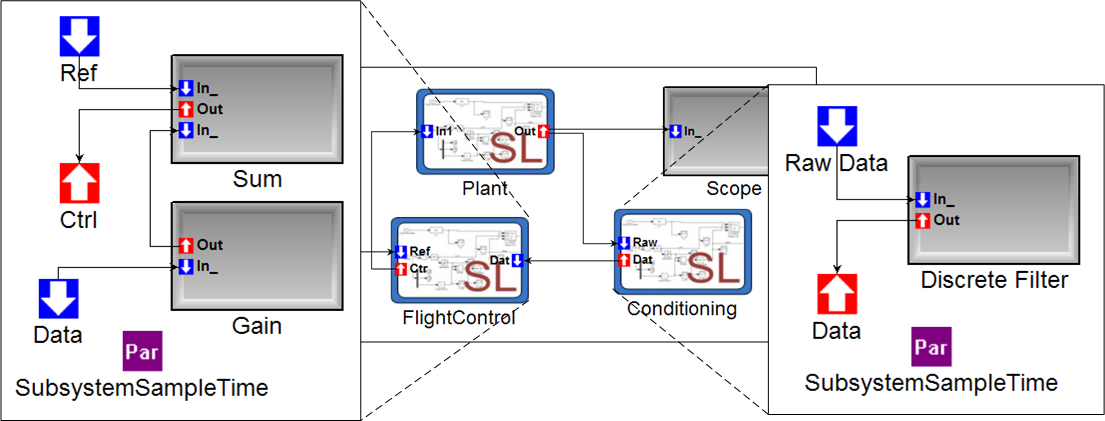
\includegraphics[width=0.9\columnwidth]{diagrams/esmol_design.png}
   \caption{ESMoL-imported functional models of the Simulink design.}
   \label{fig:esmol_design}
\end{figure}

Fig. \ref{fig:sl_design} shows a simple top-level Simulink design for our feedback loop along with the imported ESMoL model (Fig. \ref{fig:esmol_design}).  The ESMoL model is a structural replica of the original Simulink, only endowed with a richer software design environment and tool-provided APIs for navigating and manipulating the model structure in code.  A model import utility provides the illustrated function.

\subsection{Software Architecture (SwA)}

\begin{figure}
	\centering
   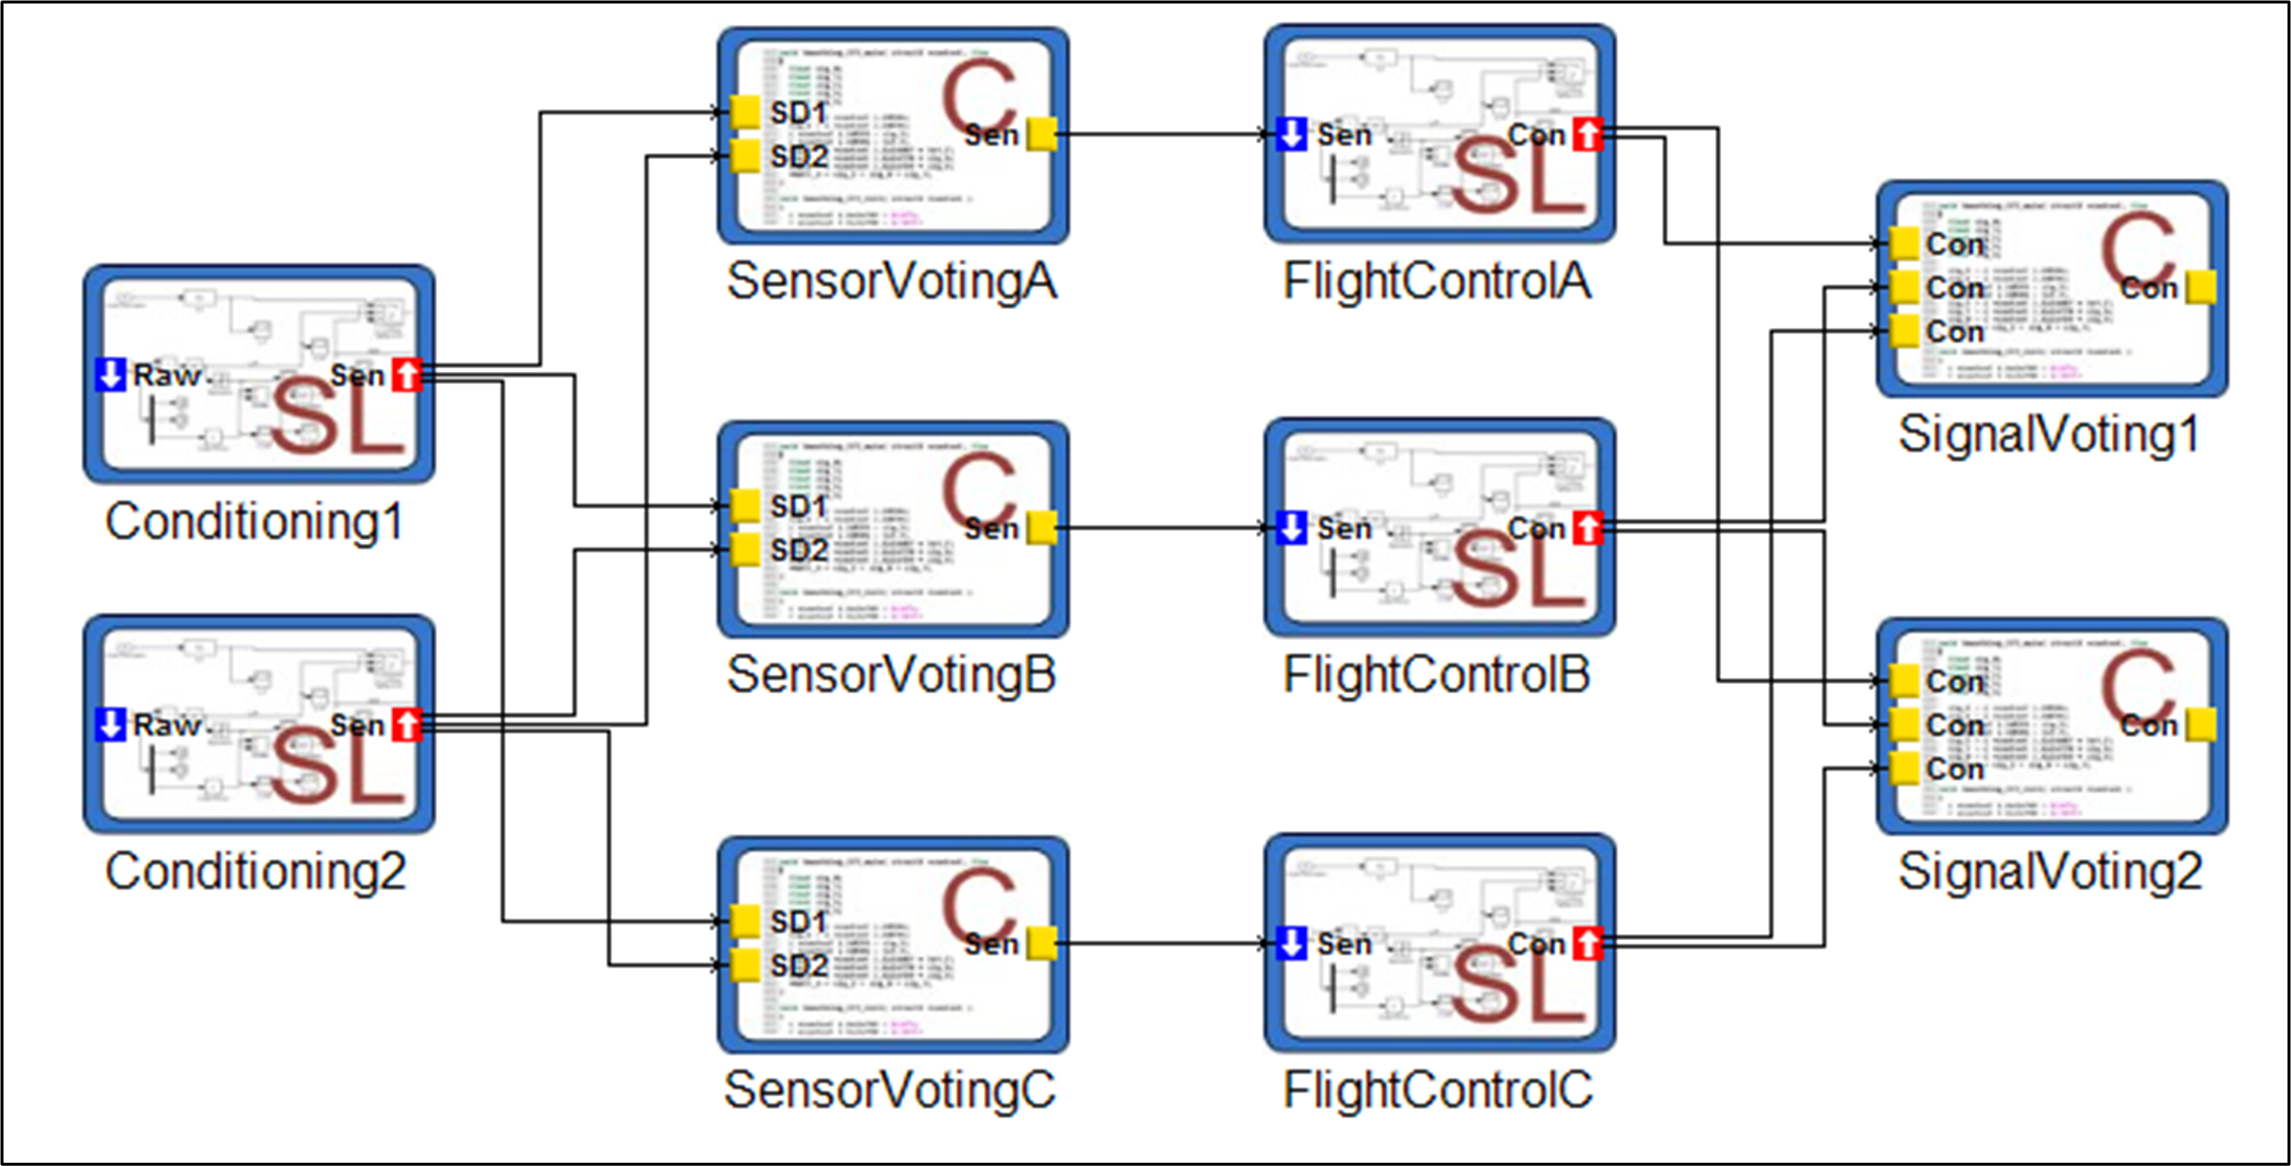
\includegraphics[width=0.7\columnwidth]{diagrams/tmr_arch.png}
   \caption{The architecture diagram defines logical interconnections, and gives finer control over instantiation of functional units.}
   \label{fig:tmr_arch}
\end{figure}

The software architecture model describes the logical interconnection of functional blocks.  In the architecture language a component may be implemented by either a Simulink Subsystem or a C function.  They are compatible at this level, because here their model elements represent the code that will finally implement the functions.  These units are modeled as blocks with ports, where the ports represent parameters passed into and out of C function calls.  The semantics for architecture model connections is that of sending and receiving messages using time-triggered communication.  

Fig. \ref{fig:tmr_arch} shows the architecture diagram for our TMR model.  Instances of the functional blocks from the Simulink model are augmented with C code implementing replicated data voting.

\subsection{Hardware Architecture (HwA)}

\begin{figure}
	\centering
   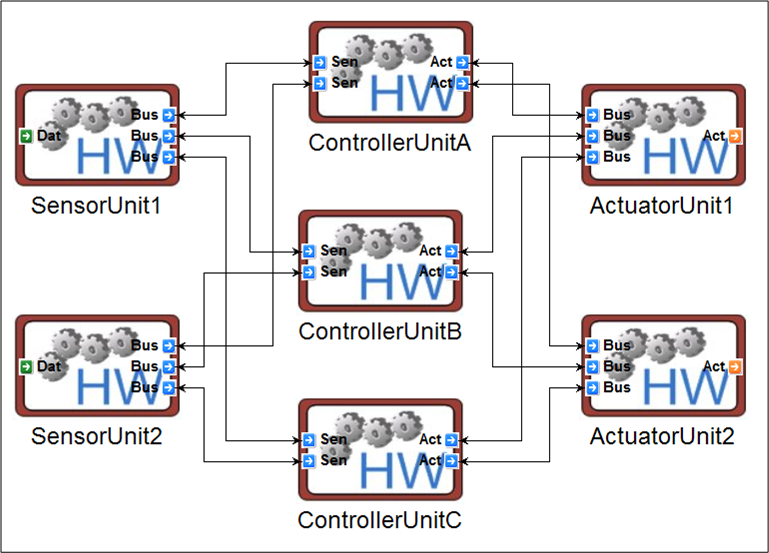
\includegraphics[width=0.75\columnwidth]{diagrams/tmr_hardware.png}
   \caption{Overall hardware layout for the TMR example.}
   \label{fig:tmr_hardware}
\end{figure}

Hardware configurations are explicitly modeled in the platform language.  Platforms are defined hierarchically as hardware units with ports for interconnections. Primitive components include processing nodes and communication buses.  Behavioral semantics for these networks come from the underlying time-triggered architecture.  The platform provides services such as deterministic execution of replicated components and timed message-passing.  Model attributes for hardware also capture timing resolution, overhead parameters for data transfers, and task context switching times.

\begin{figure}
	\centering
   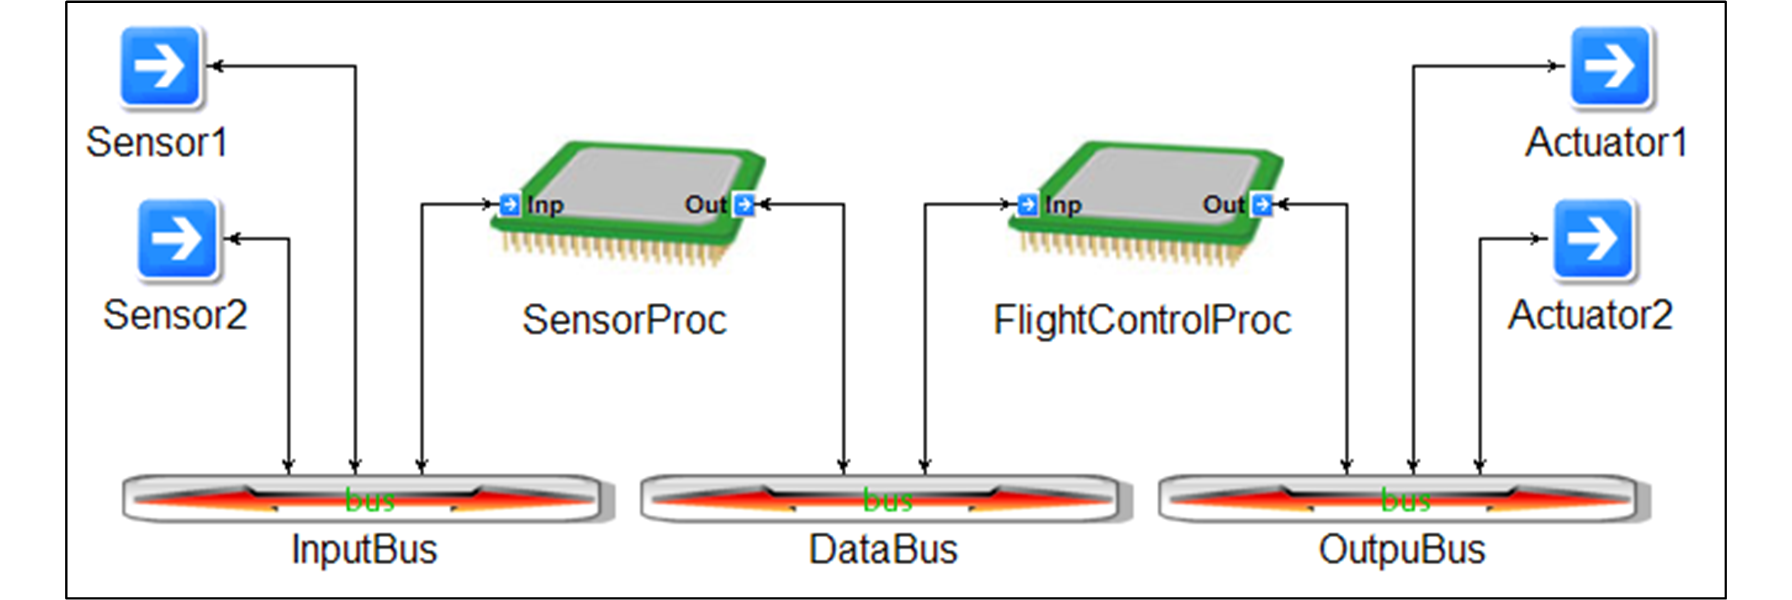
\includegraphics[width=0.8\columnwidth]{diagrams/platformex.png}
   \caption{Detail of hardware model for controller units.}
   \label{fig:platformex}
\end{figure}

Figs. \ref{fig:tmr_hardware} and \ref{fig:platformex} show model details for redundant hardware elements.  Each controller unit is a private network with two nodes and three independent data buses.
Sensor voting and flight control function instances will be deployed to the controller unit networks.

\subsection{Deployment Models (CD, SY, DPL)}

\begin{figure}
	\centering
   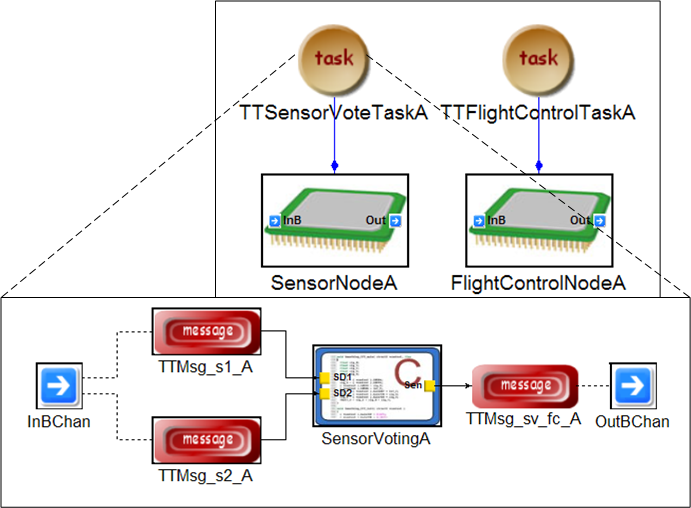
\includegraphics[width=0.55\columnwidth]{diagrams/tmr_deploy.png}
   \caption{Deployment model: task assignment to nodes and details of task definition.}
   \label{fig:tmr_deploy}
\end{figure}

A common graphical language captures the grouping of architecture components into tasks.  In ESMoL a task executes on a single processing node at a single periodic rate.  All components within the task execute synchronously.  Data sent between tasks takes the form of messages in the model.  Whether delivered locally (same processing node) or remotely, all inter-task messages are scheduled for delivery.  ESMoL uses logical execution time semantics found in time-triggered languages such as Giotto~\cite{henzinger01giotto} -- message delivery is scheduled after the deadline of the sending task, but before the release of the receiving tasks.  In the TT model of computation receivers assume that their data is available at task release time.  Tasks never block, but execute with whatever data is available each period.

Deployment concepts, tasks running on processing nodes and messages sent over data buses, are modeled as shown in Fig. \ref{fig:tmr_deploy}.  Most of the model elements shown here are actually references to elements defined in the architecture and platform models.  Model interpreters generate platform-specific code and analysis artifacts directly from the deployment models.

%%% OLD STUFF %%%%%%%%%%%%%%%%%%%%%%%%%%%%%%%%%%%%%%%%%%%%%%%%%%%%%%%%%%%%%%%%%%%%%%%%%%%%%



%\subsection{Code generators and synthesis tools}
%Model-based development is a high-level activity, i.e. programming with models instead of an algorithmic language. Therefore we need to generate executable code from the models. With proper infrastructure the generator could be more than just a model-to-code translator; it could be a code 'synthesizer' yielding low-level code from higher-level specifications. Synthesis differs from translation as it may search during the code generation process. For instance, on platforms with fixed-point arithmetic, the synthesizer could determine appropriate scaling factors for each operational step in a dataflow model based on known value ranges for inputs and outputs and the available fixed-point precision.

%Generating code from dataflow and Statechart models is a well-defined and solved problem, and there are many actual implementations. Code synthesis from higher-level models, however, is an active area of research with many open questions regarding code efficiency and correctness.

%\subsection{Verification and analysis}
%Verification and analysis are an inseparable part of the development process for high-confidence systems. There are many well-known verification techniques and tools; however, we must stress two concerns here: (1) verification tools often operate on models (i.e. abstractions of the system), not on detailed code and (2) verification results are meaningful only if model transformations from design models into analysis models or into code are correct: Properties must be carried over by the transformation with no addition of any artifacts extending behavior of the generated code beyond that of the model.

%Verification of model translators and construction of verification-based tools is an active area of research. Correctness of a model transformations is a very complex problem, but some early results indicate promising directions \cite{ananth:2006}: instead of proving correctness for a transformation in general, one can show that a particular instance of a transformation preserves the properties of interest and conclude that the properties hold for the input of the transformation.

%Another promising direction is a connection between models and the generated code. We are working on extending the code generator to carry forward model-level information to the generated code (as annotations) that provide help for the code-level verifier to check model-level properties on the code. This connection could potentially be used to improve performance, as the verifier could reason using higher-level abstractions than those immediately available from the code.  Other relevant work includes distributed modeling and verification tools like BIP~\cite{BasuBozgaSifakis07}, which strives for separation of concerns using a layered behavior model.

%

\section{Existing Tools: Simulink to TTA}
%\begin{figure}
%	\centering
%   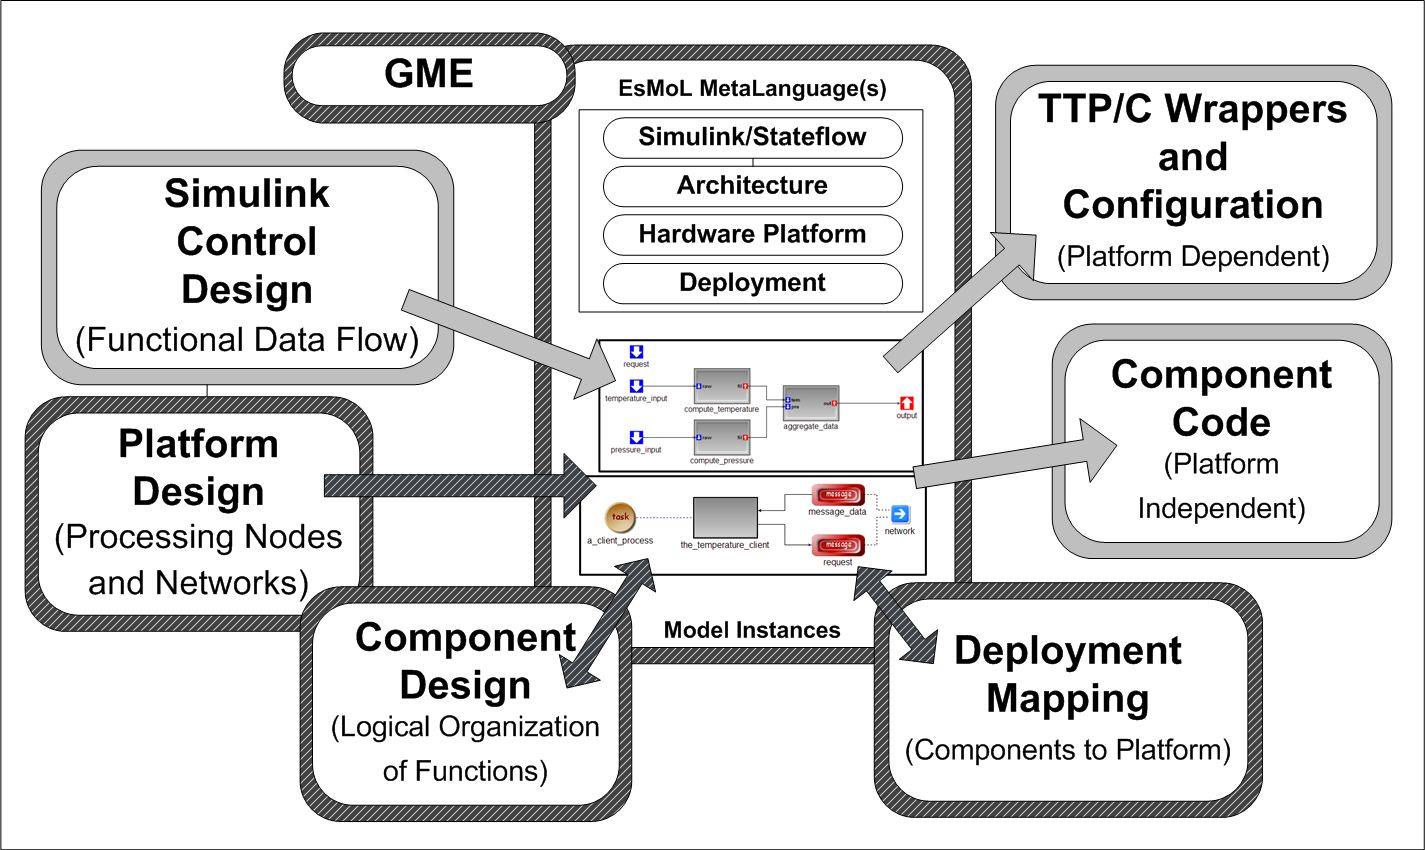
\includegraphics[width=0.55\columnwidth]{diagrams/usecase1.png}
%   \caption{Stage 1. Model interpreters automatically import Simulink and Stateflow control designs and synthesize code. Users directly enter and edit platform models, design software architecture, and create deployments using the Generic Modeling Environment (GME).}
%   \label{fig:uc1}
%\end{figure}

%Fig. \ref{fig:uc1} shows the tool flow for the existing tool chain.  
Control designs in Simulink are integrated using a graphical modeling language describing software architecture.  Components within the architecture are assigned to tasks, which run on nodes in the platform.  

\subsection{Integration Details}

\begin{figure}
	\centering
	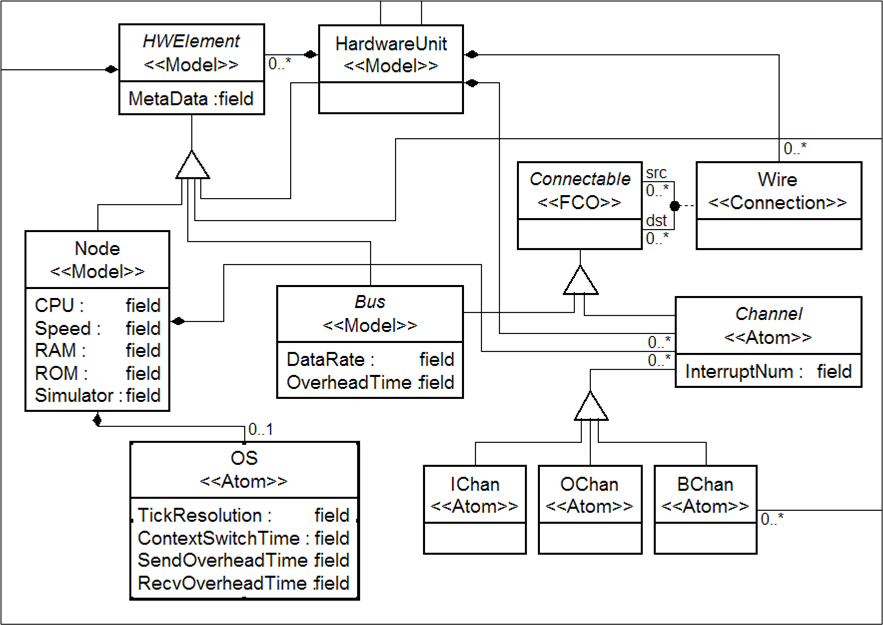
\includegraphics[width=0.75\columnwidth]{diagrams/platform.png}
	\caption{Platforms. This metamodel describes a simple language for modeling the topology of a time-triggered processing network.  A sample platform model is included.}
	\label{fig:platform}
\end{figure}

The Simulink and Stateflow sublanguages of our modeling environment are described elsewhere, though the ESMoL language changes many of the other design concepts from older languages described by Neema~\cite{KS:ISIS-04-505}.

In our toolchain we created a number of code generators. In the construction of the two main platform-independent code generators (one for Simulink-style models and another one for Stateflow-style models), we have used a higher-level approach based on graph transformations \cite{isis:great}. This approach relies on an assumption that (1) models are typed and attributed graphs with specific structure (governed by the metamodel of the language) and (2) executable code can be produced as an abstract syntax graph (which is then printed directly into source code). This graph transformation-based approach allows a higher-level representation of the translation process, which lends itself to algorithmic analysis of the transformations.

\begin{figure}
	\centering
	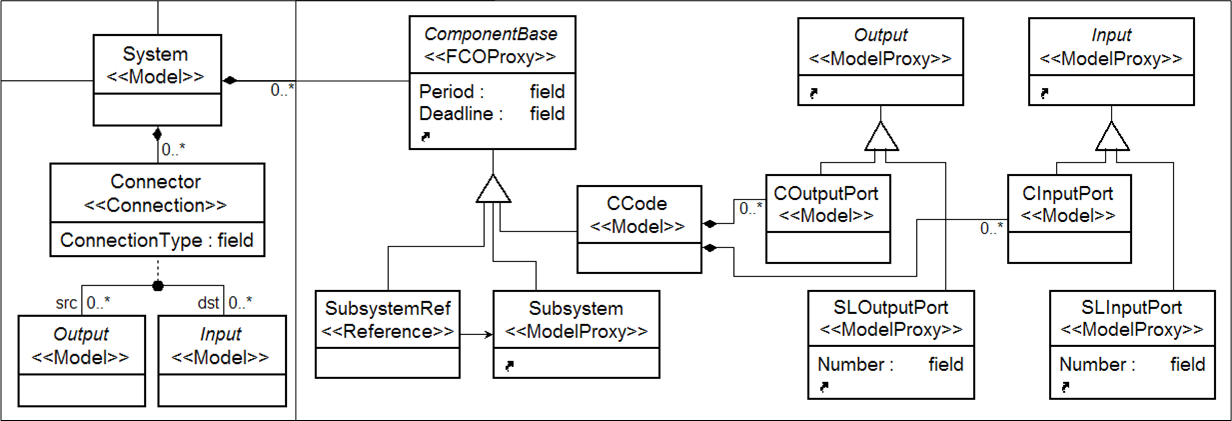
\includegraphics[width=0.9\columnwidth]{diagrams/arch_lang.png}
	\caption{Architecture Metamodel. Architecture models use Simulink subsystems or C code functions as components, adding attributes for real-time execution. The Input and Output port classes are typed according to the implementation class to which they belong.}
	\label{fig:arch}
\end{figure}

The models in the example, and the metamodels described in the sequel were created using the ISIS Generic Modeling Environment tool (GME)~\cite{isis:gme}.  GME allows language designers to create stereotyped UML-style class diagrams defining metamodels.  The metamodels are instantiated into a graphical language, and metamodel class stereotypes and attributes determine how the elements are presented and used by modelers.  The GME metamodeling syntax may not be entirely familiar to the reader, but it is well-documented elsewhere~\cite{karsai:mic}. Class concepts such as inheritance can be read analogously to UML.  Class aggregation represents containment in the modeling environment, though an aggregate element can be flagged as a port object.  In the modeling environment a port object will also be visible at the next higher level in the model hierarchy, and available for connections.  The dot between the Connectable class and the Wire class represents a line-style connector in the modeling environment.

High-confidence systems require platforms that provide services and guarantees for needed properties, e.g. fault containment, temporal firewalls, etc. These critical services (like partitioning) should be provided by the platform and not re-implemented from scratch by system developers~\cite{alberto:2002}.  Note that the platform also defines a 'Model of Computation' \cite{Lee:M97/11}. An MoC governs how the concurrent objects of an application interact (i.e. synchronization and communication), and how these activities unfold in time. The simple platform definition language shown in Fig. \ref{fig:platform} contains relationships and attributes for describing a time-triggered network. 

\begin{figure}
	\centering
%	\subfigure[Tasks contain Components and associate with Nodes.]{
	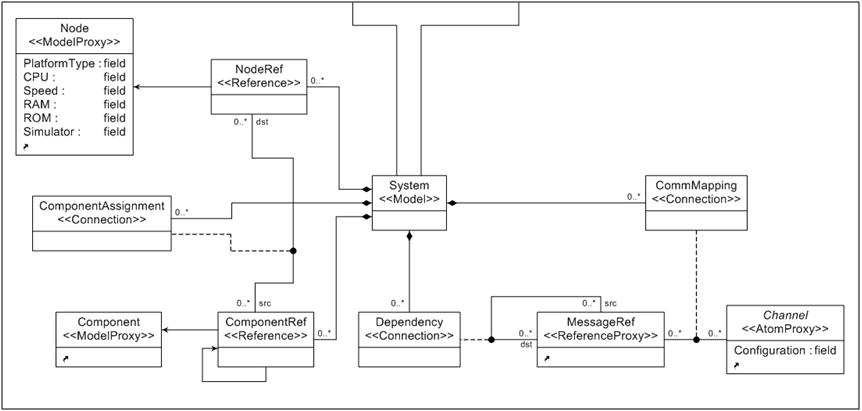
\includegraphics[width=\columnwidth]{diagrams/depnew.png}
%	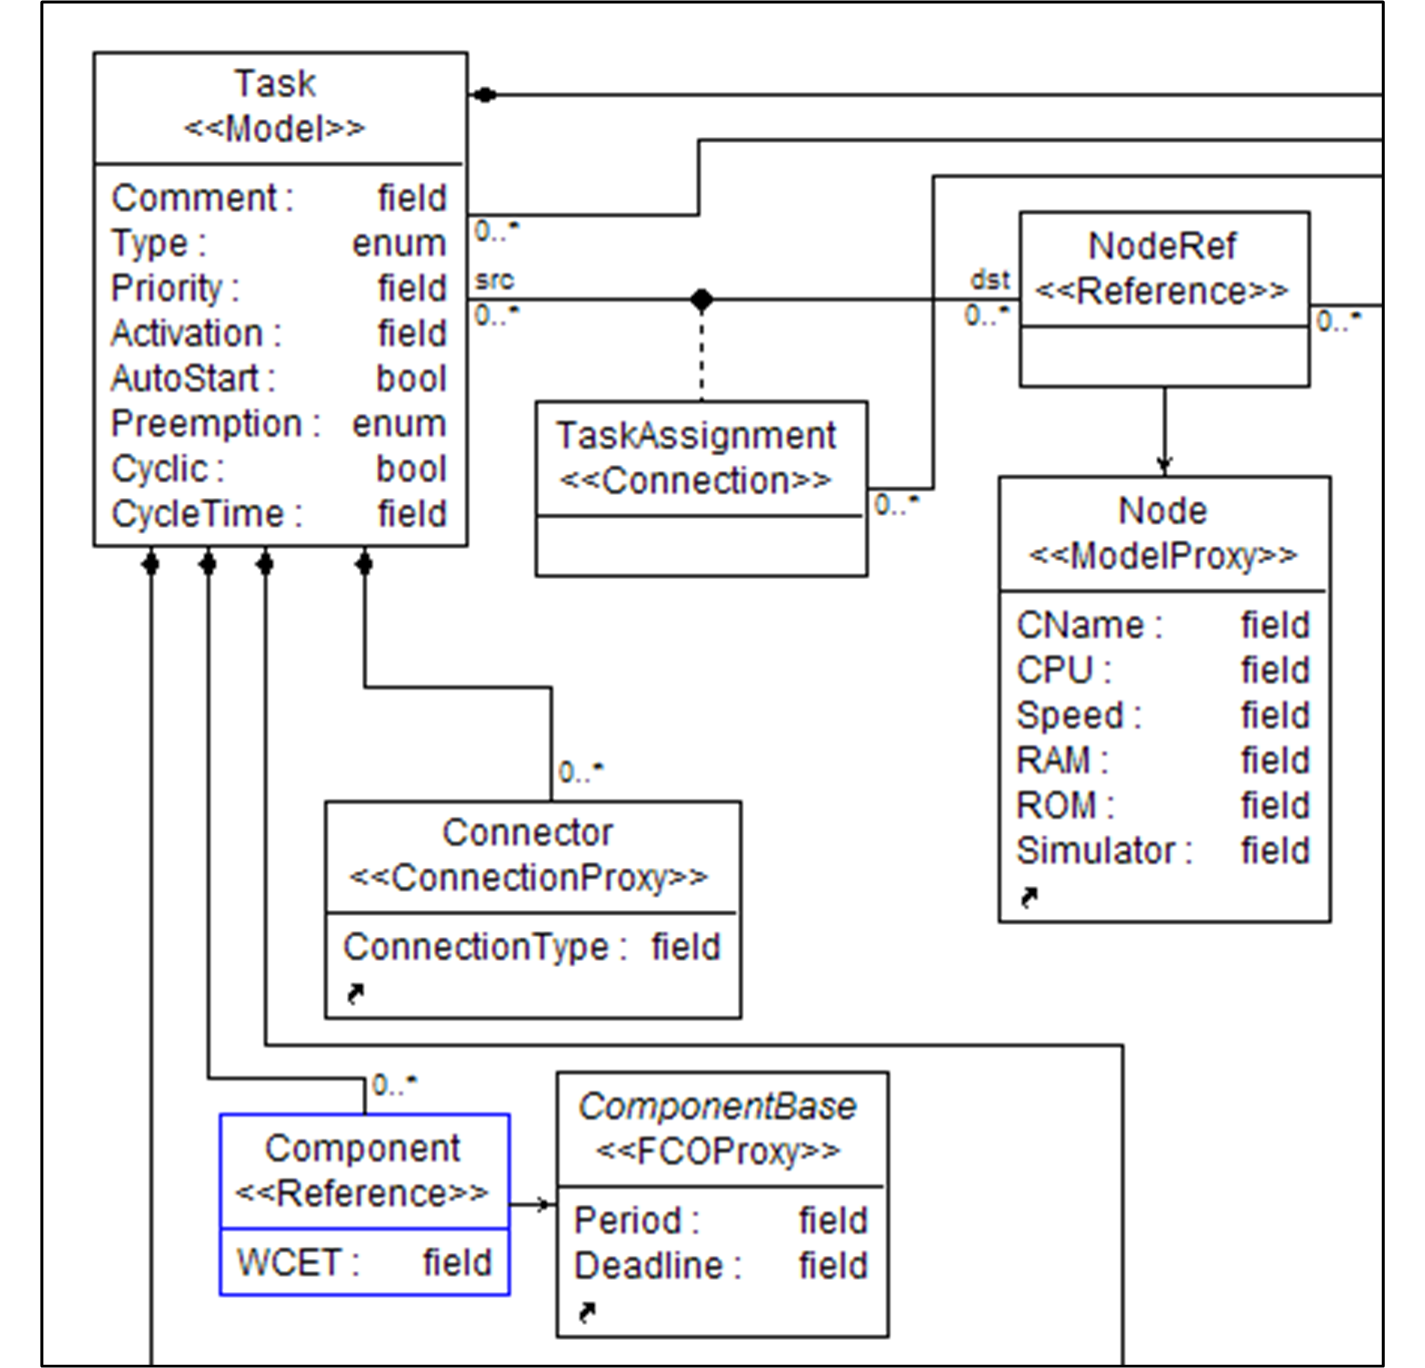
\includegraphics[scale=1]{diagrams/depcompnew.png}
%	\label{fig:depcomp}
%	}
%	
%	\subfigure[InputPorts and OutputPorts from Simulink connect to Messages.]{
%	%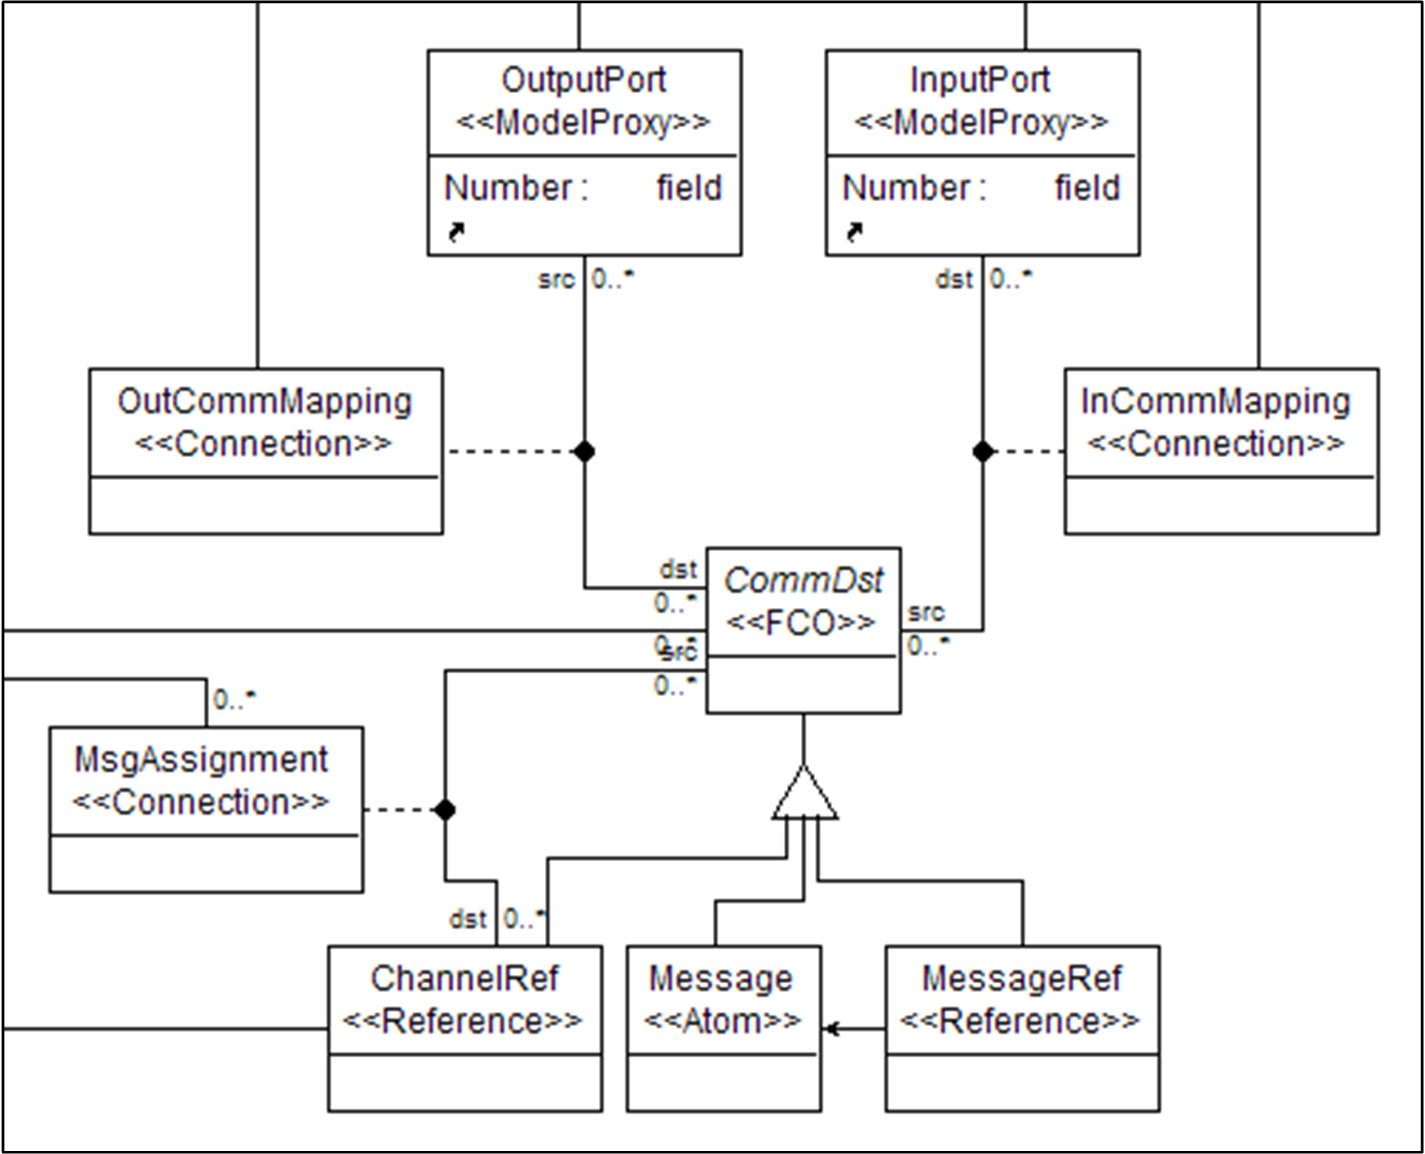
\includegraphics[width=0.9\columnwidth]{diagrams/depportnew.png}
%	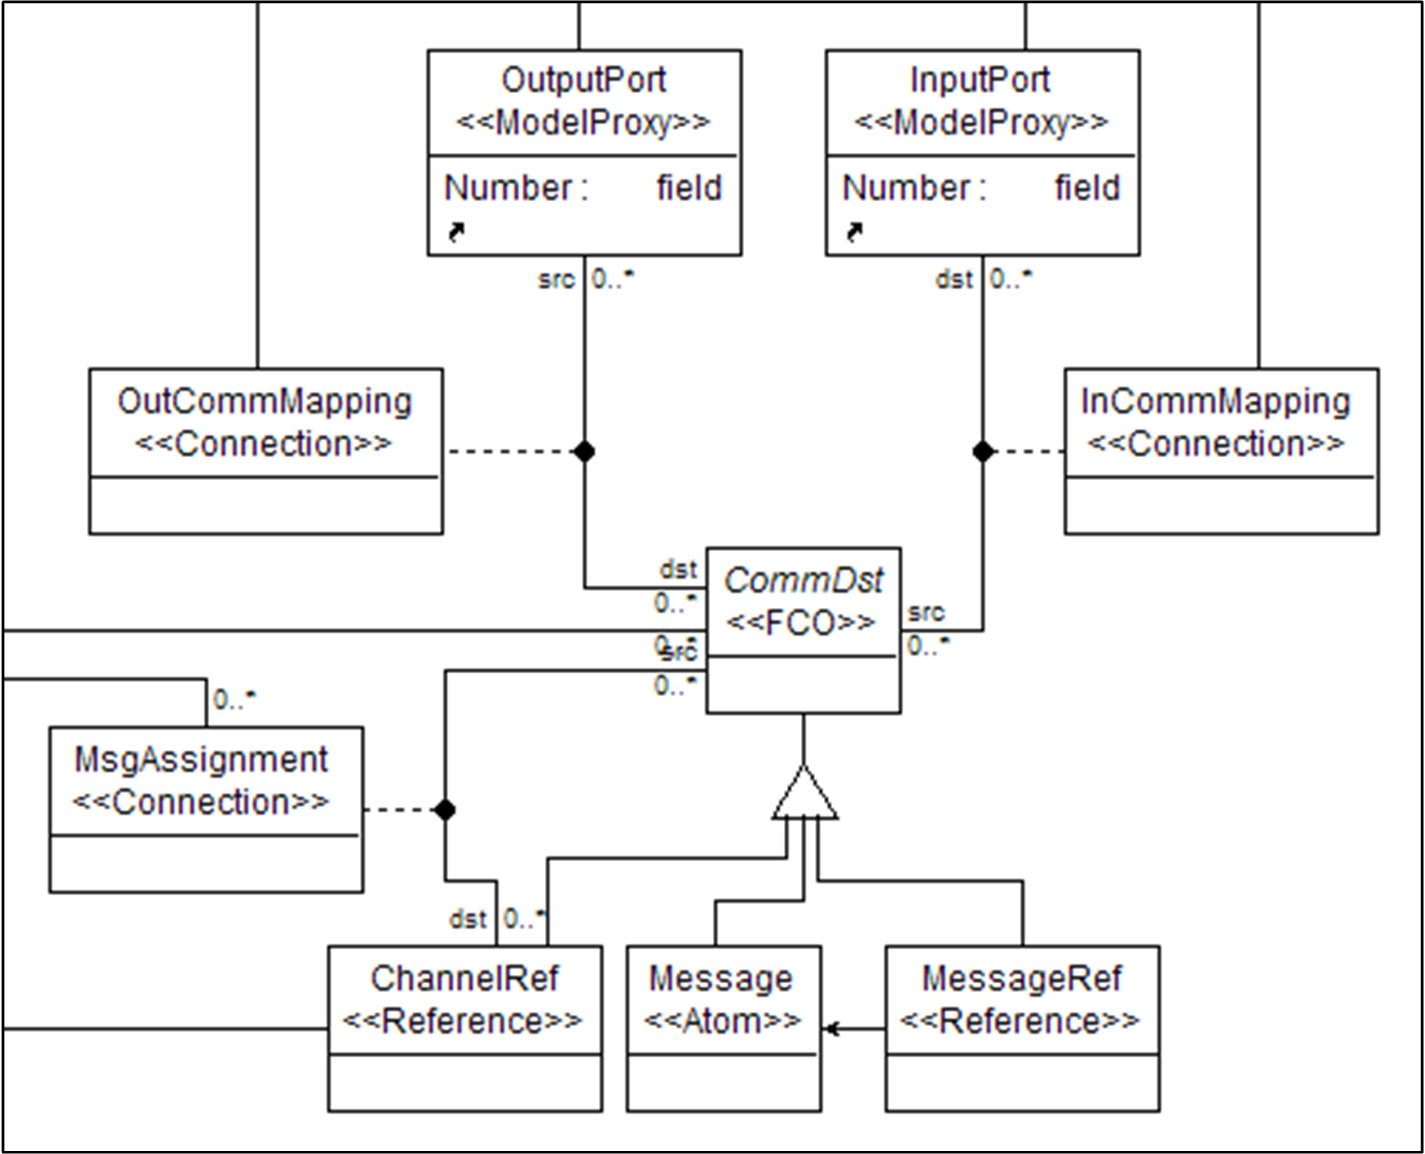
\includegraphics[scale=0.9]{diagrams/depportnew.png}
%	\label{fig:depport}
%	}
	\caption{Details from deployment sublanguage.}
	\label{fig:depnew}
\end{figure}

Similarly, Fig. \ref{fig:arch} describes the software architecture language. The Connector element models communication between components.  Semantic details of communication interactions remain abstract in this logical architecture -- the platform model must be specified and associated in order to completely specify the interactions (though in this version we only offer synchronous and time-triggered communications).

Deployment models capture the assignment of Components (and Ports) from the Architecture to Platform Nodes (and Channels).  Additional implementation details (e.g. worst-case execution time) are represented here for platform-specific synthesis.  Fig. \ref{fig:depnew} shows the relevant modeling concepts.  Simulink objects SLInputPort and SLOutputPort are assigned to Message objects, which represent the marshaling of data to be sent on a Bus.

%\subsection{Current and Future Work}

%Simulink/Stateflow model import and code generation are the most mature features of the toolchain, so the described features are fairly well supported.  Ongoing work extends the number of Simulink blocks which can be synthesized by the code generator, and adds the ability to import Matlab functions embedded in the Simulink designs.
%
%

\section{Under Development: Platform-specific simulation, generic hardware, and scheduling}

%\begin{figure}[h]
%	\centering
%   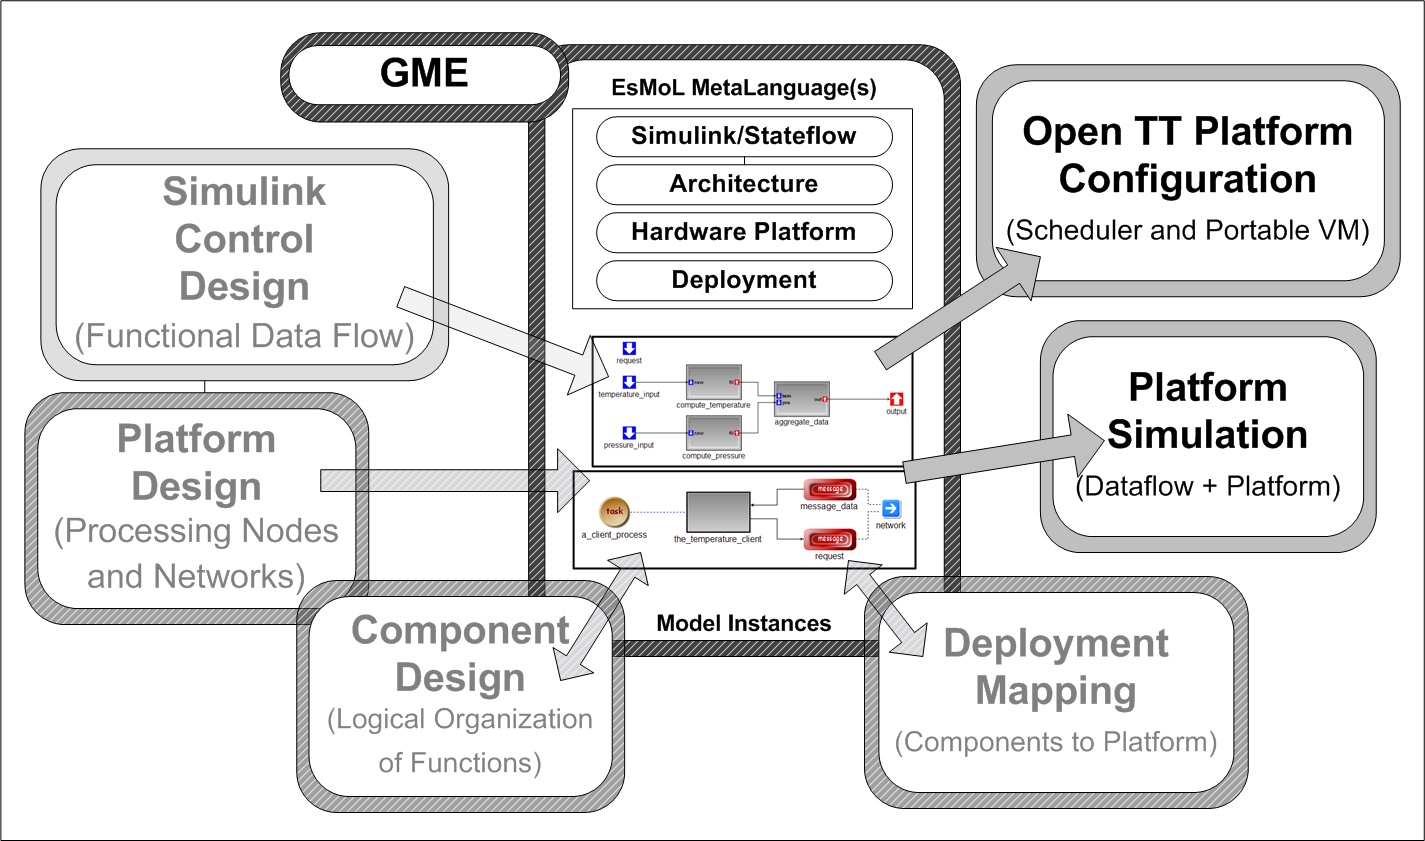
\includegraphics[width=0.55\columnwidth]{diagrams/usecase2.png}
%   \caption{Designers can synthesize simulations which include platform effects. Wrapper and configuration synthesis for time-triggered hardware can also be easily adapted to generate code and configuration for an open time-triggered (TT) platform and related scheduling tools. }
%   \label{fig:uc2}
%\end{figure}

%Fig. \ref{fig:uc2} shows the tool flow for features under development.  
A control system designer initially uses simulation to check correctness of the design.  Software engineers later take code implementing control functions and deploy it to distributed controllers.  Concurrent execution and platform limitations may introduce new behaviors which degrade controller performance and introduce errors.  Ideally, the tools could allow the control functions to be re-simulated with appropriate platform effects.

%\begin{figure}[h]
%	\centering
%   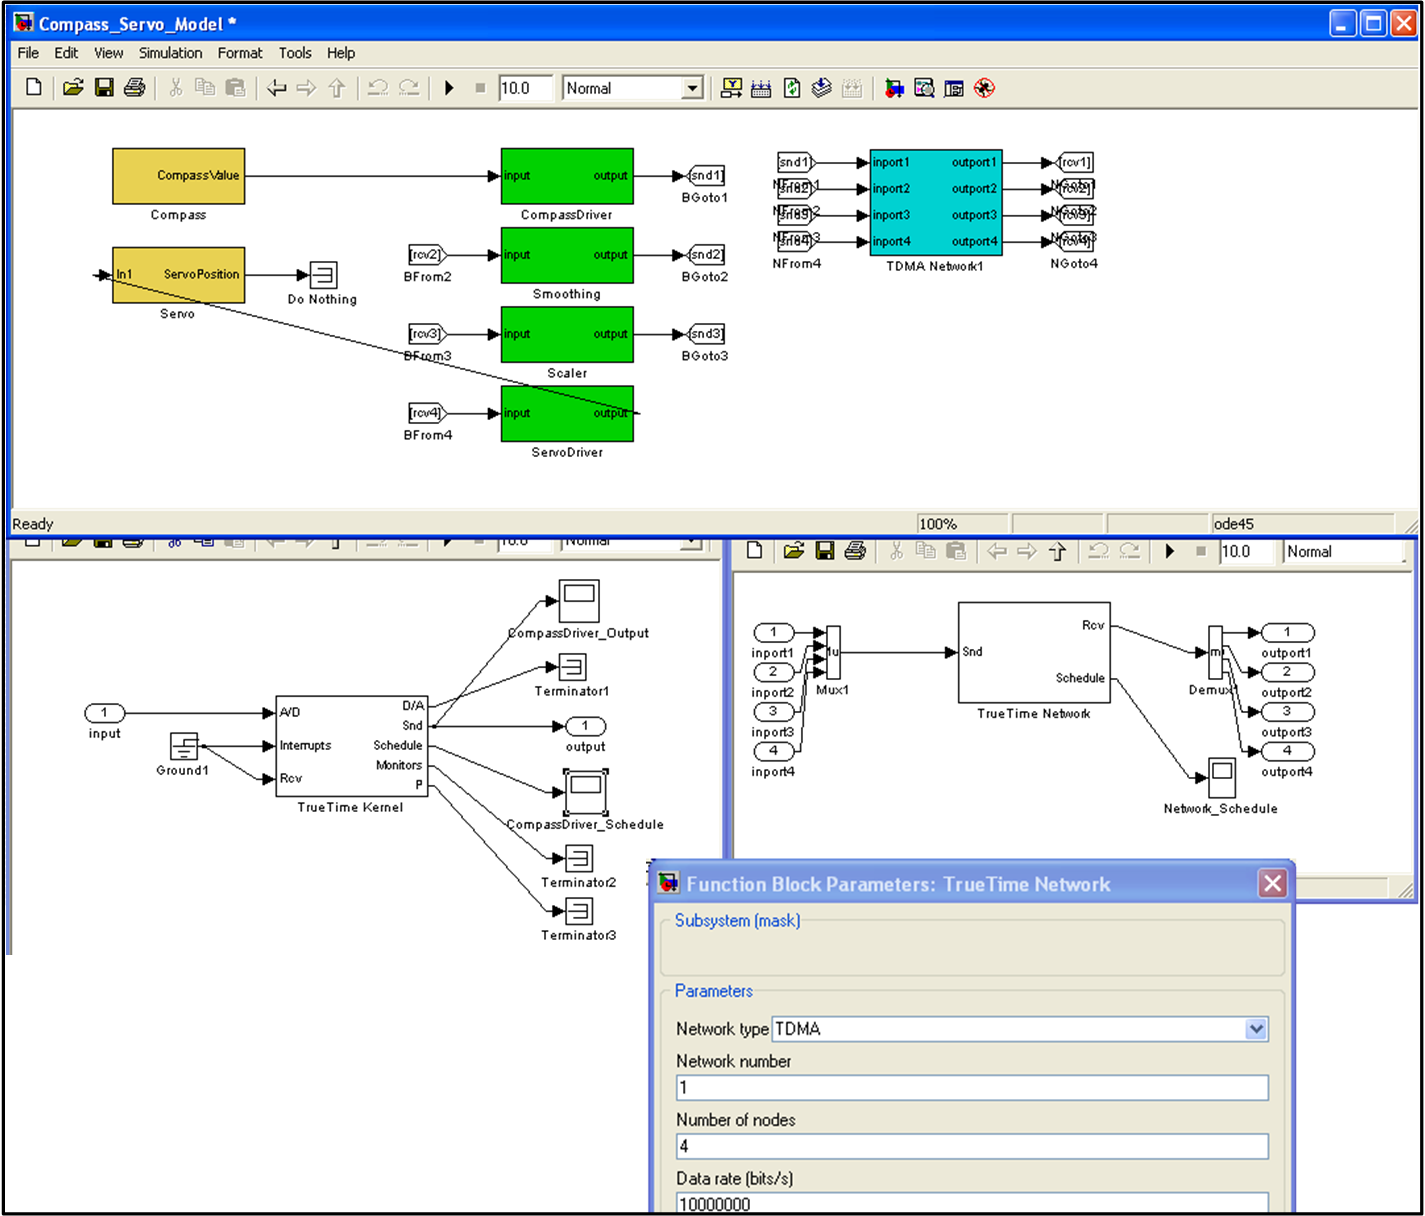
\includegraphics[width=0.5\columnwidth]{diagrams/truetime.png}
%   \caption{TrueTime Simulink model with parameter window.}
%   \label{fig:truetime}
%\end{figure}

The TrueTime simulation environment~\cite{TrueTime} provides Simulink blocks modeling processing nodes and communication links.  Tasks can execute existing C code or invoke subsystems in Simulink models.  Task execution follows configured real-time scheduling models, with communication over a selected medium and protocol.  TrueTime models use a Matlab script to associate platform elements with function implementations.  A platform-specific re-simulation requires this Matlab mapping function, and in our case also a periodic schedule for distributed time-triggered execution.  Both of these can be obtained by synthesis from ESMoL models.  
%Fig. \ref{fig:truetime} shows an example TrueTime model.

After resimulation follows synthesis to a time-triggered platform. In order to use generic computing hardware with this modeling environment, we created a simple, portable time-triggered virtual machine to simulate the timed behavior of a TT cluster~\cite{RT_Thesis} on generic processing hardware.  Since the commercial TT cluster and the open TT virtual machine both implement the same model of computation, synthesis differences amount to management of structural details in the models.  The open VM platform is limited to the timing precision of the underlying processor, operating system, and network, but it is useful for testing.

For both steps above the missing link is schedule generation.  In commercial TTP platforms, associated software tools perform cluster analysis and schedule generation.  For resimulation and deployment to an open platform, an open schedule generation tool is required.  To this end we created a simple schedule generator using the Gecode constraint programming library~\cite{gecode}.  The scheduling approach implements and extends the work of Schild and W{\"u}rtz~\cite{sw:offlinescheduling}.  Configuration for the schedule generator is also generated by the modeling tools.

\subsection{Integration Details}

To configure TrueTime or the scheduler, the important details lie in the deployment model.  Tasks and Messages must be associated with the proper processing nodes and bus channels in the model.  The ISIS UDM libraries~\cite{UDM} provide a portable C++ API for creating interpreters to navigate models and extract the relevant information.  See Fig. \ref{fig:depnew} for the relevant associations.  Model navigation in these intepreters must maintain the relationships between processors and tasks and between buses and messages.  Scheduler configuration also requires extraction of all message sender and receiver dependencies in the model.

%\subsection{Current and Future Work}

%This development stage has had working prototypes and demos for each of the described elements.  The features are being adapted to recent language changes, integrated more fully, and polished.
%
%

\section{Designs in Progress: Requirements and model updates}


%\begin{figure}
%	\centering
%   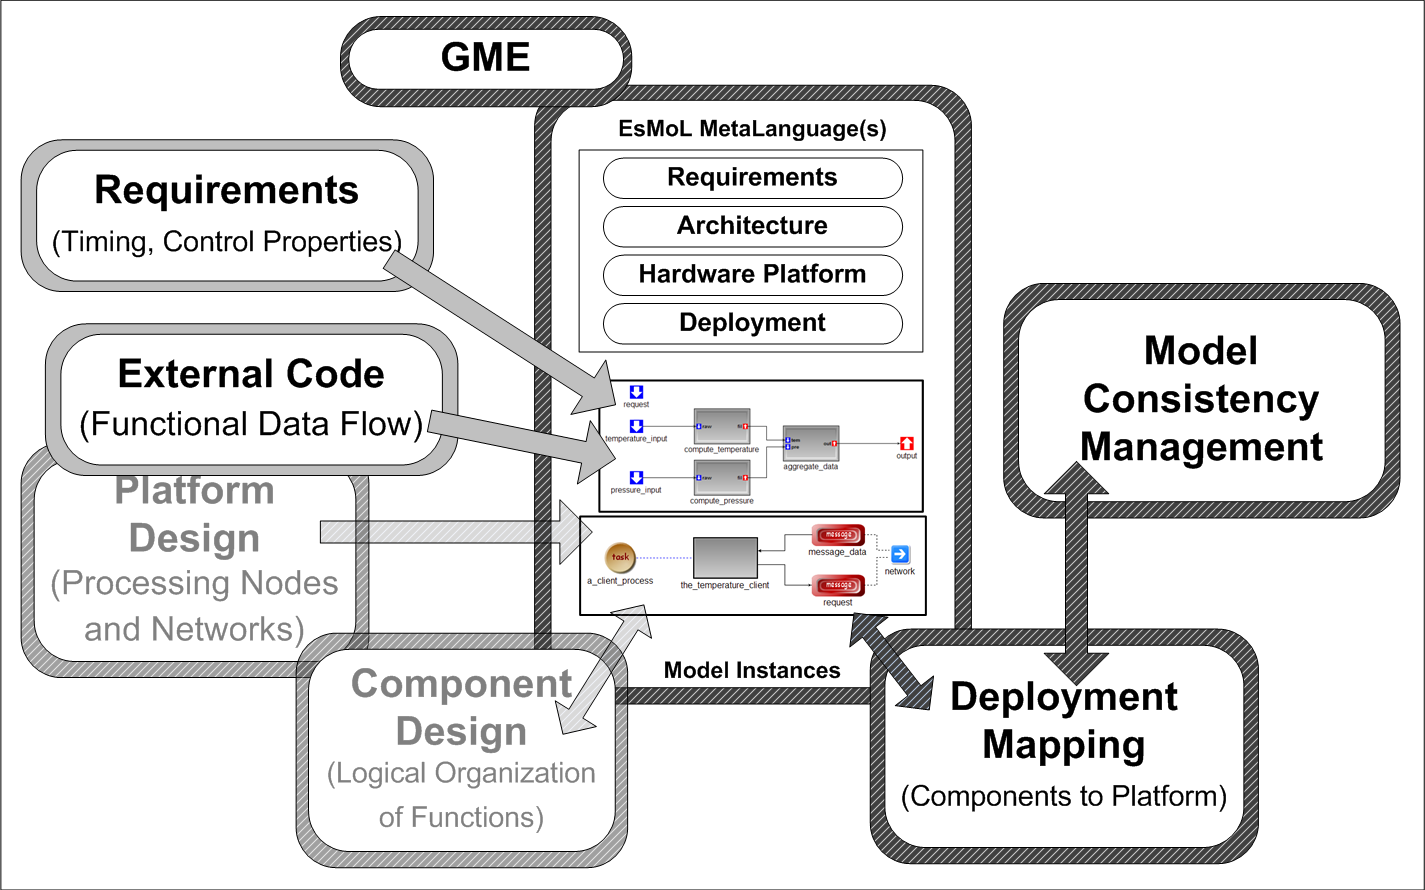
\includegraphics[width=0.55\columnwidth]{diagrams/usecase3.png}
%   \caption{equirements modeling and automated management of deployment models when functional and platform models change.  }
%   \label{fig:uc3}
%\end{figure}

%Fig. \ref{fig:uc3} depicts features of designs in progress.  
Many types of requirements apply to real-time embedded control systems design. Embedded systems are heterogeneous, so requirements can include constraints on control performance, computational resources, mechanical design, and reliability, to name a few things. Formal safety standards (e.g. DO-178B~\cite{DO178B}) impose constraints on the designs as well as on the development process itself.  Accordingly, current research has produced many techniques for formalizing requirements (e.g. ground models in abstract state machines~\cite{Borger} or Z notation~\cite{Z2}).  Models could be used to incorporate formal requirements into other aspects of the design process.  During analysis, requirements may appear as constraints in synthesized optimization problems or conditions for model checking.  Requirements can also be used for test generation and assessment of results.

Management of model updates is also essential. As designs evolve engineers and developers reassess and make modifications.  Changes to either the platform model or functional aspects of the design may invalidate architecture and deployment models created earlier.  Some portions of the dependent models will survive changes.  Other parts needing changes must be identified.  Where possible, updates should be automated.

\subsection{Integration Details}

\begin{figure}
	\begin{minipage}{2.25in}
	\centering
   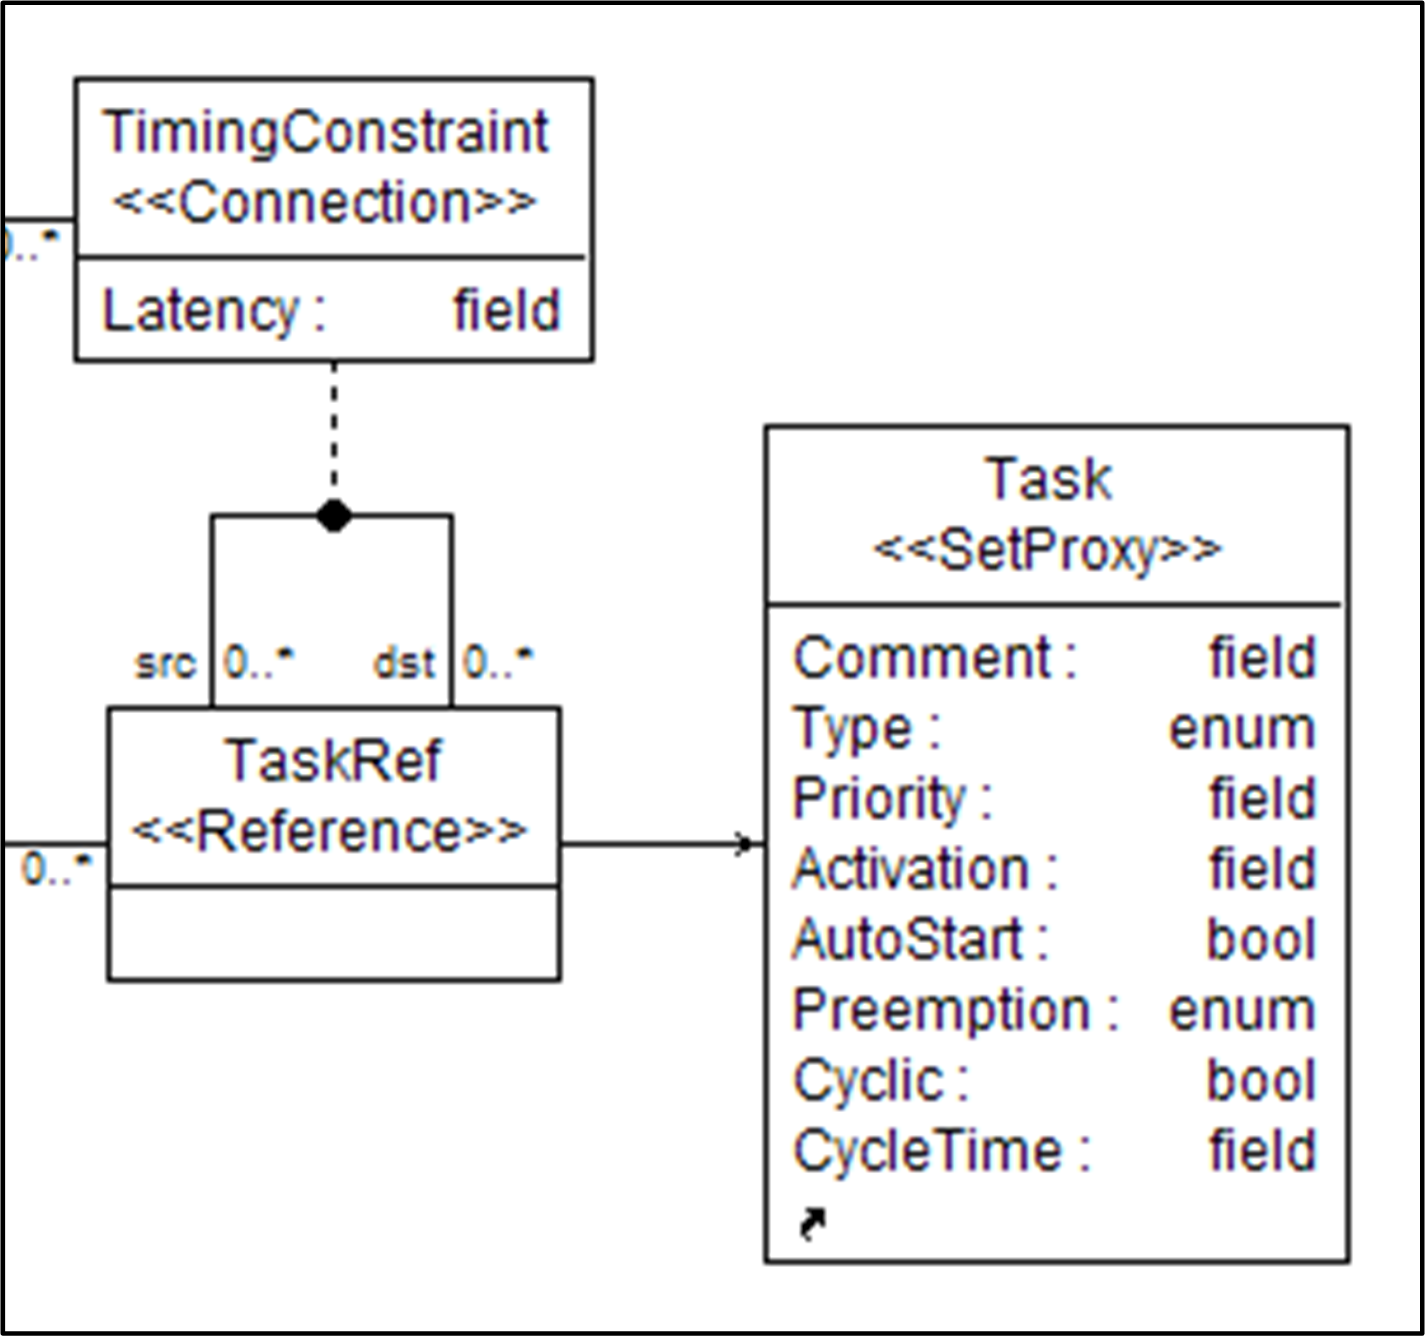
\includegraphics[width=0.75\columnwidth]{diagrams/reqs.png}
   \caption{Latencies are timing constraints between task execution times. }
   \label{fig:reqs}
\end{minipage}
\hspace{0.125in}
	\begin{minipage}{2.375in}
	\centering
   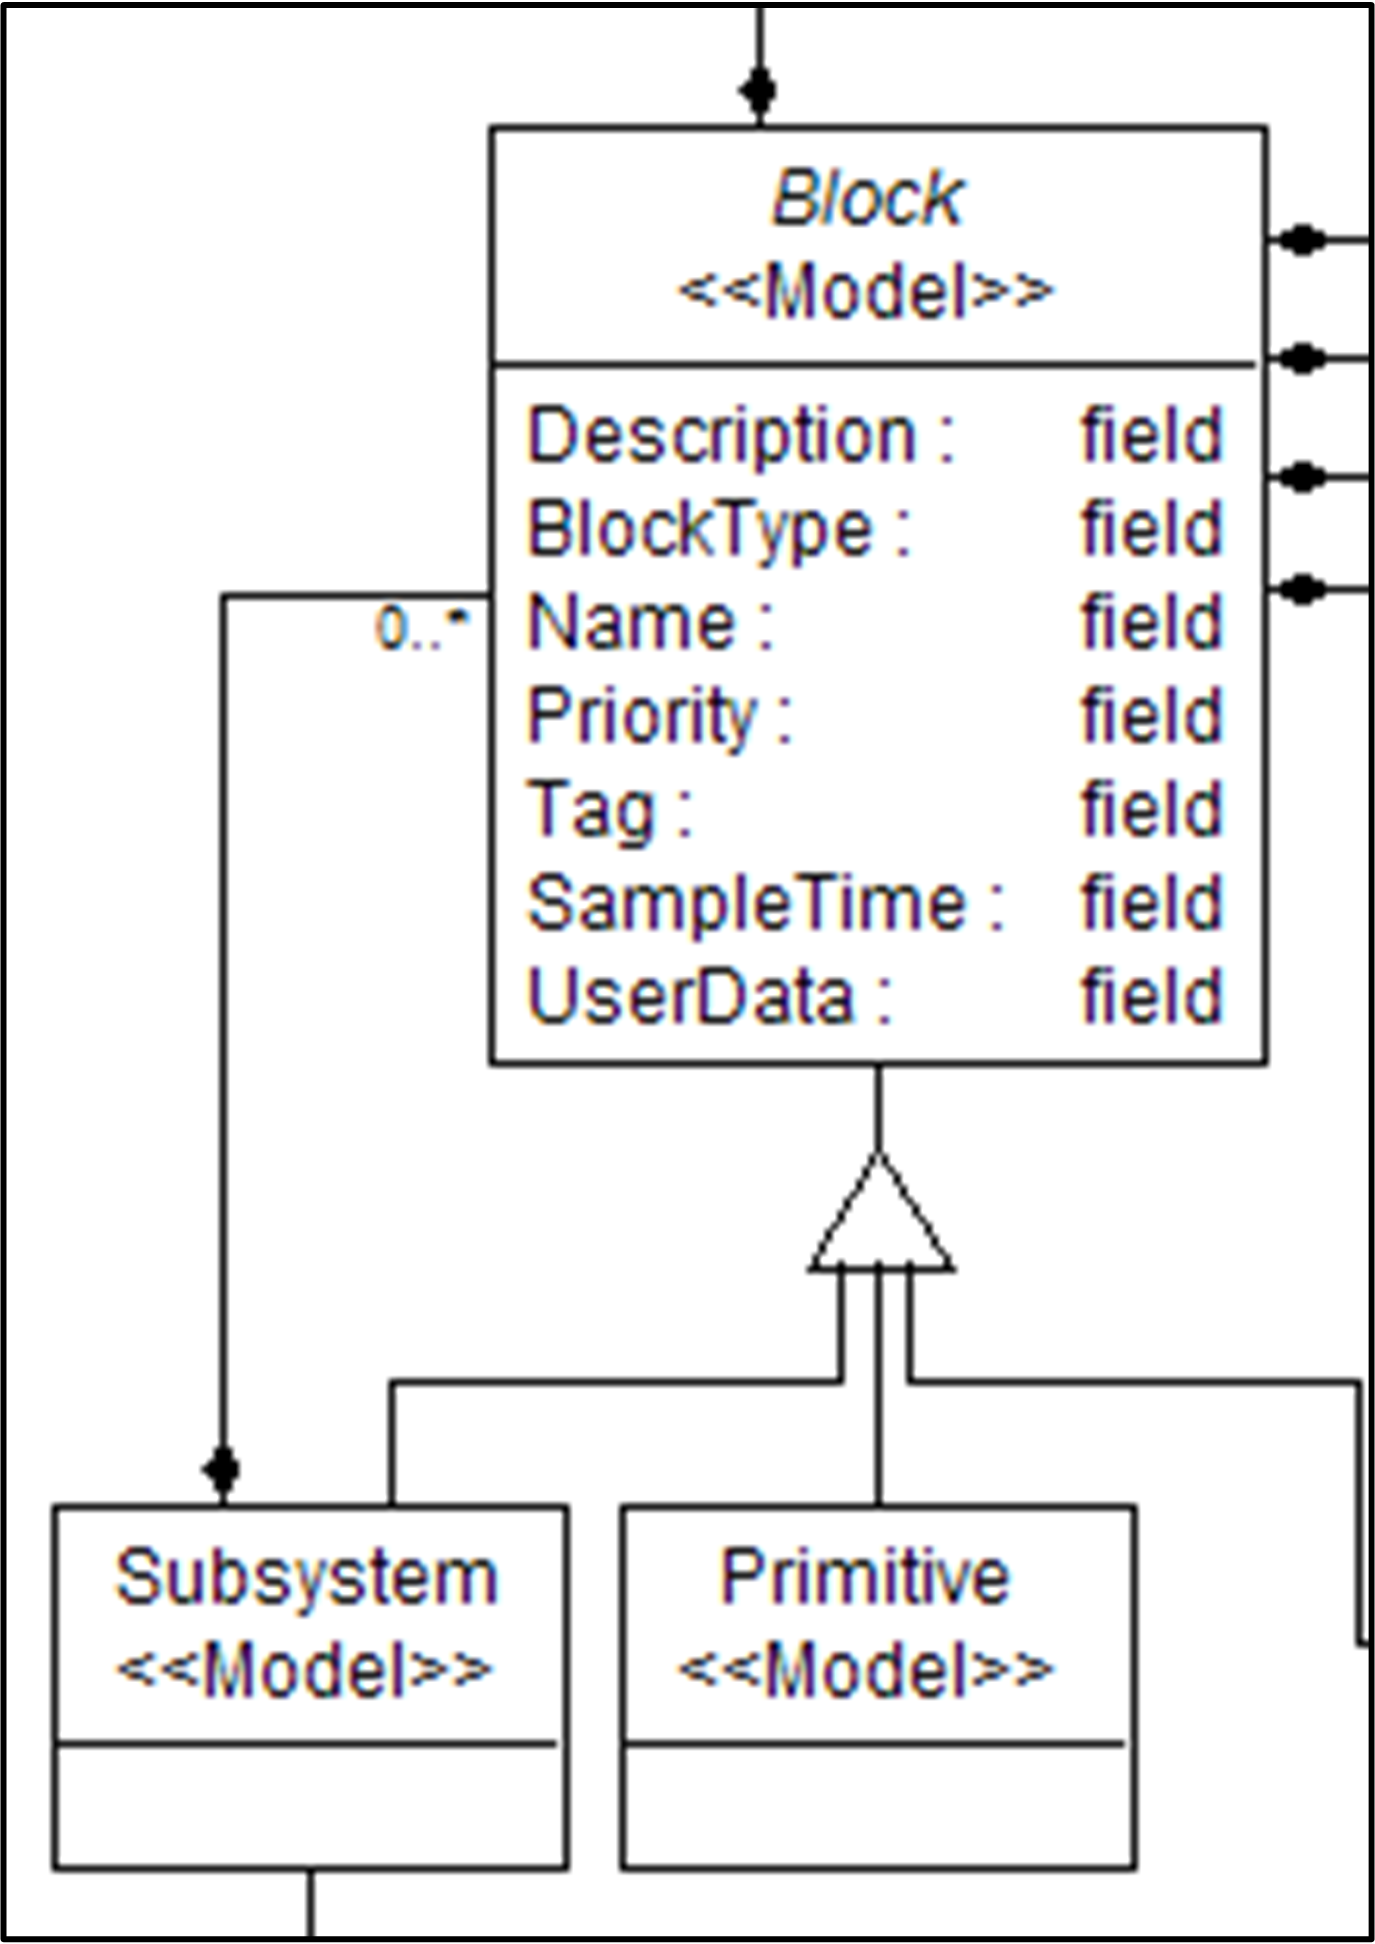
\includegraphics[width=0.65\columnwidth]{diagrams/userdata.png}
   \caption{Simulink's UserData field can help manage model changes occuring outside the design environment. }
   \label{fig:userdata}
   \end{minipage}
\end{figure}

The requirements sublanguage is in design, and so is light on details. Fig. \ref{fig:latency} shows an example model with latency requirements between tasks, and Fig. \ref{fig:reqs} shows the modeling language definition.  This simple relationship can be quantified and passed directly to the schedule solver as a constraint.  Ideally a more sophisticated requirements language could capture the syntax and semantics of an existing formal requirements tool.  Some candidate languages and approaches are currently under consideration for inclusion in the framework.  

\begin{figure}
	\centering
   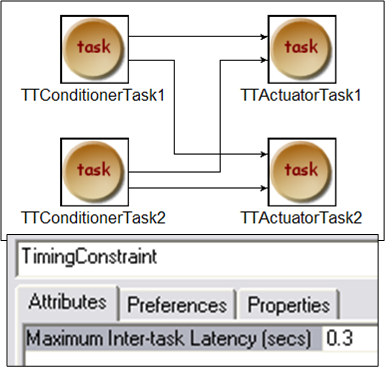
\includegraphics[width=0.55\columnwidth]{diagrams/latency.png}
   \caption{Example of task latency spec for sample model, with detail of timing attribute value specified on model links.}
   \label{fig:latency}
\end{figure}

To track model changes we propose to use the Simulink UserData field to store unique tags when the models are imported.  During an update operation tags in the control design can be compared with previously imported tags in the model environment.  Fig. \ref{fig:userdata} shows the UserData attribute from our Simulink sublanguage, corresponding to the actual attribute in Simulink blocks.  
%Successful updating relies on restriction of the hierarchy.  Allowing the modeling environment to track changes at any depth in the hierarchy can allow some algorithmically difficult situations. With restricted depth lower level details are abstracted away, leaving only changes that would affect the software architecture or deployment relationships.  This imposes some reasonable discipline on control designers, who must organize the top level of their Simulink designs into functional blocks.  Another benefit of this structural requirement is added clarity of designs.
To handle issues arising from topology concerns, we require control designers to group top-level functionality into subsystems and place a few restrictions on model hierarchy in deployment models.

%\subsection{Current and Future Work}

%All of these language elements and features are in the early stages of design or prototype, though work has been done to flesh out many of the required details.
%
%

\section{Wishlist: Expanded semantics, implementation generation, and verification}

Many exciting possibilities loom on the horizon for this tool chain construction effort.  We briefly describe some forward-looking concepts currently in discussion for the tools.  %The fourth stage of development is depicted in Fig. \ref{fig:uc4}.

%\begin{figure}
%	\centering
%   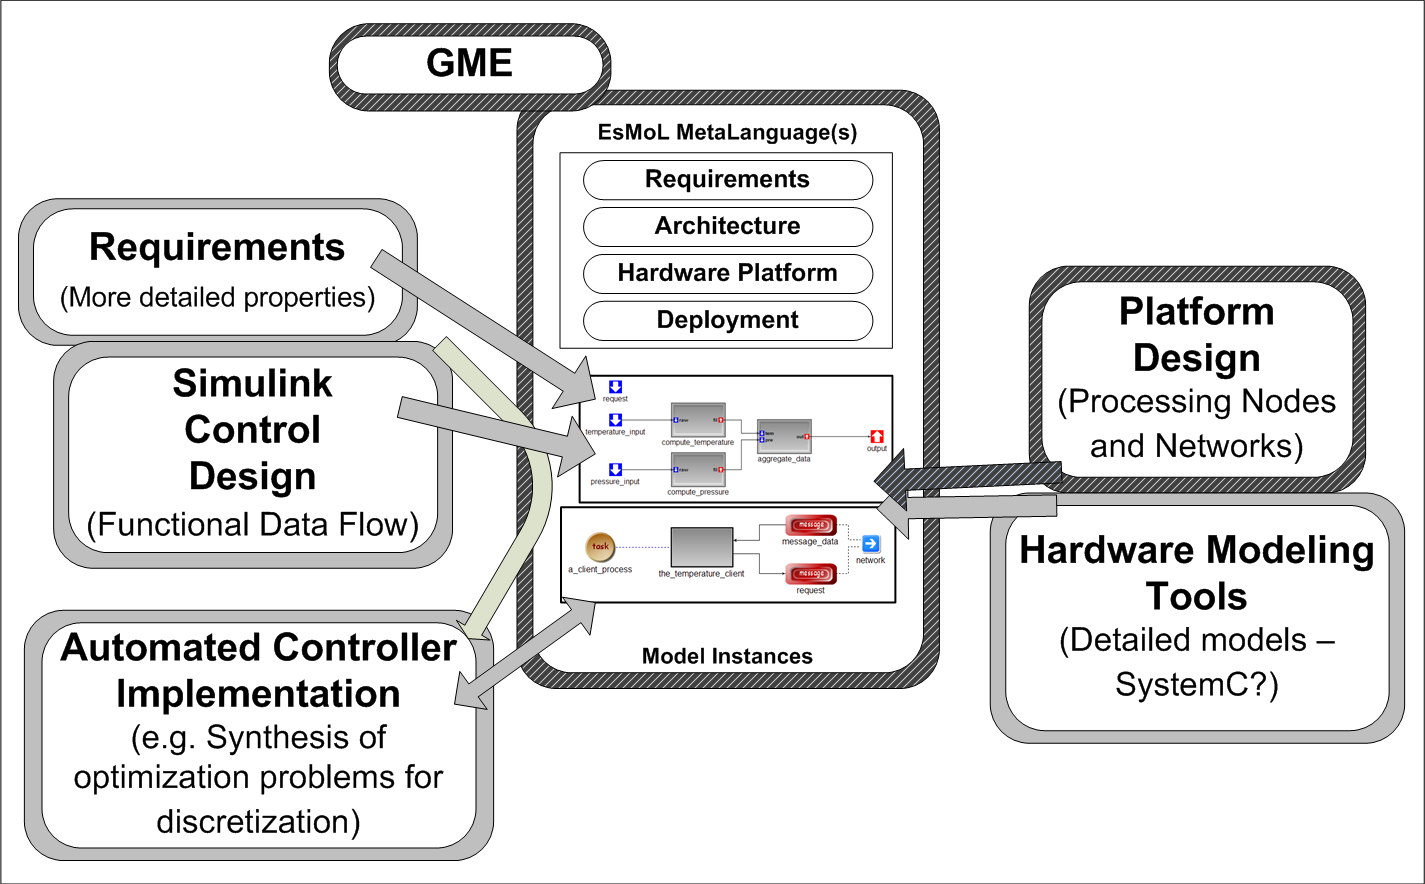
\includegraphics[width=0.55\columnwidth]{diagrams/usecase4.png}
%   \caption{Stage 4. Extension of formal requirements and platform models and automated synthesis of discretized controllers.  These are wishlist items, though some preliminary experiments and designs have been made.}
%   \label{fig:uc4}
%\end{figure}

The current modeling languages describe systems which provide performance and reliability guarantees by implementing a time-triggered model of computation.  This is not adequate for many physical processes and controller platforms.  We also need provisions for event-triggered communication and components.  Event-triggered component structures give rise to interesting and useful communication patterns common in practical systems (e.g. publish-subscribe, rendezvous, and broadcast). Several research projects have explored heterogeneous timed models of computation.  Two notable examples are the Ptolemy project~\cite{ucb:ptolemy2} and the DEVs formalism and associated implementations~\cite{DEVSpp}.  More general simulation and model-checking tools for timed systems and specifications include UPPAAL~\cite{UPPAAL} and timed abstract state machines~\cite{TASM}.  We aim to identify useful design idioms from event-triggered models and extend the semantics of the modeling language to incorporate them.  Synthesis to analysis tools is also possible using model APIs.  

Safe automation of controller implementation techniques is another focus.  Control designs are often created and simulated in continuous time and arbitrary numerical precision, and then discretized in time for platforms with periodic sampling and in value for platforms with limited numeric precision.  Recent work in optimization and control offers some techniques for building optimization problems which describe valid controller implementation possibilities~\cite{LMITrunc}~\cite{LMINetwork}. Early model interpreter work aims to generate such optimization problems directly from the models.  Other interesting problems include automated generation of fixed-point scaling for data flow designs.  If integrated, tools like BIP~\cite{BasuBozgaSifakis07} provide potential for automated verification of distributed computing properties (safety, liveness, etc...).  Model representation of data flow functions, platform precision, and safety requirements could be used together for scaling calculation.
  
The addition of proper formal requirements modeling can enable synthesis of conditions for model checking and other verification tools.  Executable semantics for these modeling languages can also provide the behavioral models to be checked (see Chen~\cite{SU_TA}~\cite{SU_MT}, Gargantini~\cite{ASM_SPIN}, and Ouimet~\cite{TASM_SAT}).  Other relevant work includes integration of code-level checking, as in the Java Pathfinder~\cite{Pathfinder} or Saturn~\cite{Stanford_Saturn} tools.  Synthesis to these models must also be verified, an active area of research at ISIS~\cite{ananth:2006}.

%

\section{Acknowledgements}
This work is sponsored in part by the National Science Foundation (grant NSF-CCF-0820088) and by the Air Force Office of Scientific Research, USAF (grant/contract number FA9550-06-0312).  The views and conclusions contained herein are those of the authors and should not be interpreted as necessarily representing the official policies or endorsements, either expressed or implied, of the Air Force Office of Scientific Research or the U.S. Government.


% ---- Bibliography ----
%
\bibliographystyle{splncs}
\bibliography{aces_2008}

%\end{multicols}

\end{document}
